\chapter{Data Analysis II: Cuts and final PID}
\label{chap:data2}

As Chapter~\ref{chap:data1} covered the corrections and various calibrations to the data, this Chapter will cover the various cuts taken to improve the signal in the experimental data. Some cuts which identify the incoming beam and the event on target are the minimum cut in order to perform an analysis. The cuts pertaining to the track reconstruction quality are also required to suppress as much of the background noise as possible, most of which comes from reconstruction inefficiencies which the cuts presented here address. 



\section{Beam Particle Identification}
\label{sec:beam}

\begin{figure}[!htb]
\centering
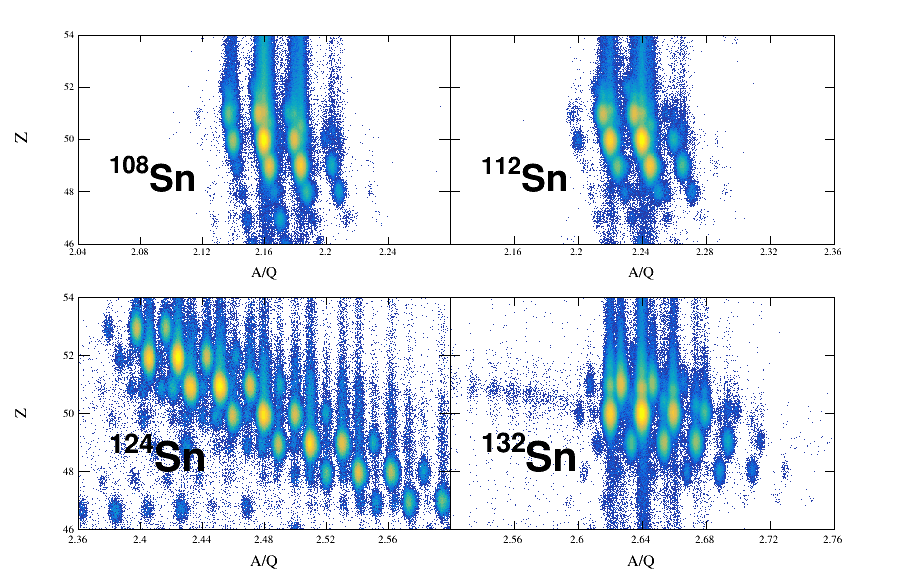
\includegraphics[width=\textwidth]{beamPID.png}
\caption{Overall beam PID for all the systems. Several contaminants other than the desired secondary beam can be seen.}
\label{fig:beampid}
\end{figure}


\begin{figure}[!htb]

     \centering
     \begin{subfigure}[b]{0.49\textwidth}
         \centering
         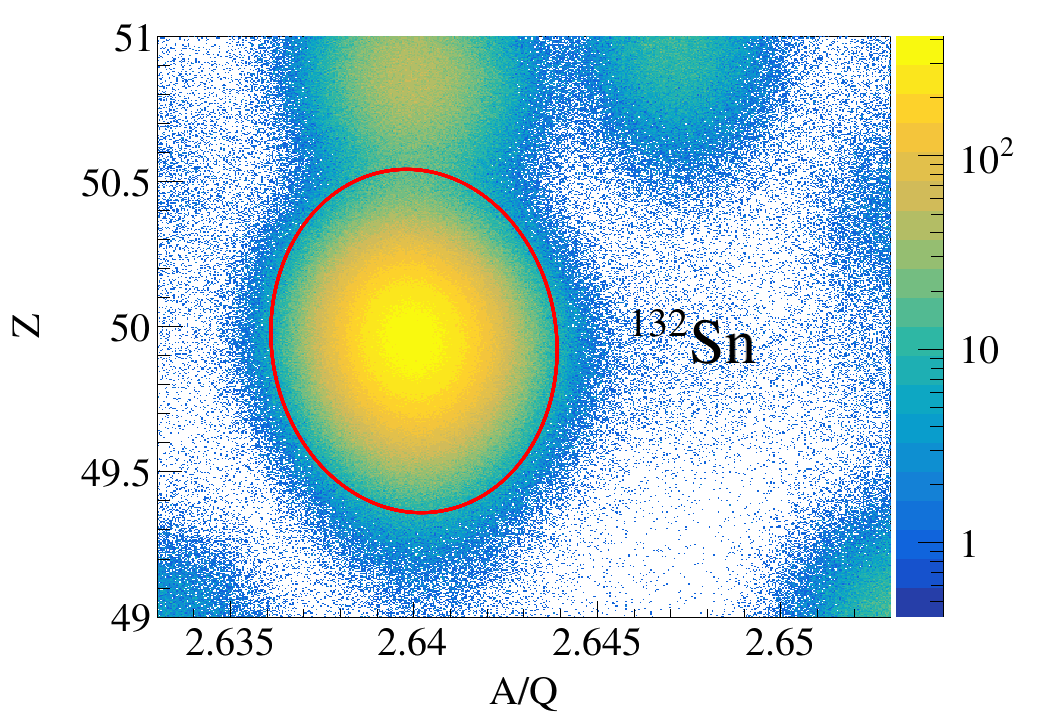
\includegraphics[width=\textwidth]{beam-Sn132.png}
         \caption{$\tin{132}{124}$ system.}
         \label{fig:beampid132}
     \end{subfigure}
     \hfill
     \begin{subfigure}[b]{0.49\textwidth}
         \centering
         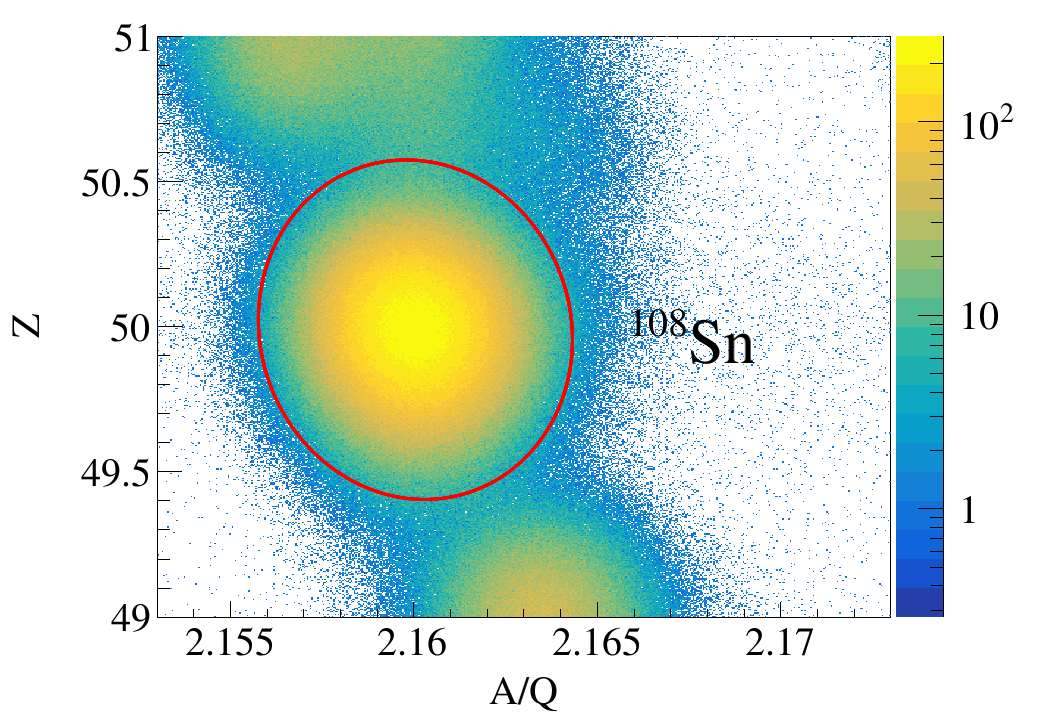
\includegraphics[width=\textwidth]{beam-Sn108.png}
         \caption{$\tin{108}{112}$ system.}
         \label{fig:beampid108}
     \end{subfigure}
        \caption{Beam PID achieved of the the neutron rich and poor systems, from analysis of the BigRIPs spectrometer \cite{jon} }
        \label{fig:beampidTwo}
\end{figure}


%Figures of beam contaminants in our beam PID line. 
%Table of beam purity reference to Jon's thesis paper
The secondary beam is produced through the projectile fragmentation of the primary beam off of a \SI{3}{\milli\metre} thick, rotating Be target \cite{inflightsep}. The resulting fragments are filtered in-flight to the desired seconary beam. The in-flight separation is handled by the BigRIPS fragment separator which is shown in Figure~\ref{fig:samuraiBeamLine}. The dipole magnets D1 and D2 act as a velocity filter, selecting on certain magnetic rigidities $\beta\rho$. Several sets of slits further purify the secondary beam quality by discarding particles which do not focus on the right focal planes. These are the areas where the particles with different velocities focus to different locations in space, which occur at F3,F5, and F7 positions.  Each beam is tracked with the remaining part of the BigRIPS spectrometer tracking system. The particle identification of each beam is achived by the TOF-B$\rho$-$\Delta$E method described in \cite{bigrips}, where the Time of Flight (TOF) information is given by the time it takes to cross two plastic scintilators at F3 and F7 focal planes, and the $\Delta$E information is given by the MUlti-Sampling Ionization Chamber (MUSIC) \cite{music}. From this method the atomic charge, Z, and mass to charge ratio, A/Q, of each particle was measured and separate species represent two-dimensional Gaussian in this space. 

Figure~\ref{fig:beampid} shows the beam PID for all the systems for events which satisfied the trigger, several contaminants other than the desired secondary beams still passed through the BigRIPS spectrometer and made it into the TPC. The beam purity of each desired secondary beam is listed in Table~\ref{tb:beams}. The desired secondary beam of interest can be selected by using an appropriate gate around the corresponding particle. Each particle gate is selected by fitting a multivariate normal distribution with two variables defined as,

\begin{equation}
  f(x,y)=\frac1{2\pi\sigma_x\sigma_y\sqrt{1-\rho^2}}\exp\left\{
  \frac{-(x - \mu_{x})^2/\sigma_x^2-(y-\mu_{y})^2/\sigma_y^2+2\rho
  xy/\sigma_x\sigma_y}{2(1-\rho^2)}\right\},
   \label{multiGauss}
\end{equation}
where x=A/Q, y=Z, $\mu$ is the mean values, and $\sigma$ are the Gaussian widths of the two variables. The gates drawn in Figure~\ref{fig:beampidTwo} are summarized in Table~\ref{beamParameters}. 

\begin{table}[!htb]
  \begin{center}
    \begin{tabular}{cccccc}
      \hline 
      Particle Type & $\mu_\mathrm{A/Q}$ & $\sigma_\mathrm{A/Q}$ & $\mu_\mathrm{Z}$ &
      $\sigma_\mathrm{Z}$ & $\rho$\\
      \hline\hline 
      ${}^{132}$Sn & 2.64 & 0.0014 & 49.95 & 0.209 & -0.052 \\
    %  $\tin{124}{112}$ & 2.24005 & 0.00150934 & 49.9906 & 0.194804 & -0.0671999 \\
    %  $\tin{112}{124}$ & 2.47995 & 0.00182327 & 49.961 & 0.214745 & -0.0742297 \\
      ${}^{108}$Sn & 2.16 & 0.0015 & 49.99 & 0.207 & -0.059 \\
      \hline
    \end{tabular}
    \caption{2D Gaussian cuts parameters for all four systems beam PID.
    \label{beamParameters}}
  \end{center}
\end{table}

Figure~\ref{fig:beampid132} shows a zoomed in view of the PID centered around the ${}^{132}$Sn beam and Figure~\ref{fig:beampid108} the ${}^{108}$Sn beam. The red lines represent the cut where particles identified inside the circle represent the beam events which are identified as the good beam events. For both ${}^{132}$Sn an ${}^{108}$Sn a 2.83$\sigma$ cut is taken around the mean values.  


\section{Edge Cuts}

\begin{figure}[!htb]

    \centering
    \begin{subfigure}[t]{0.45\textwidth}
        \centering
        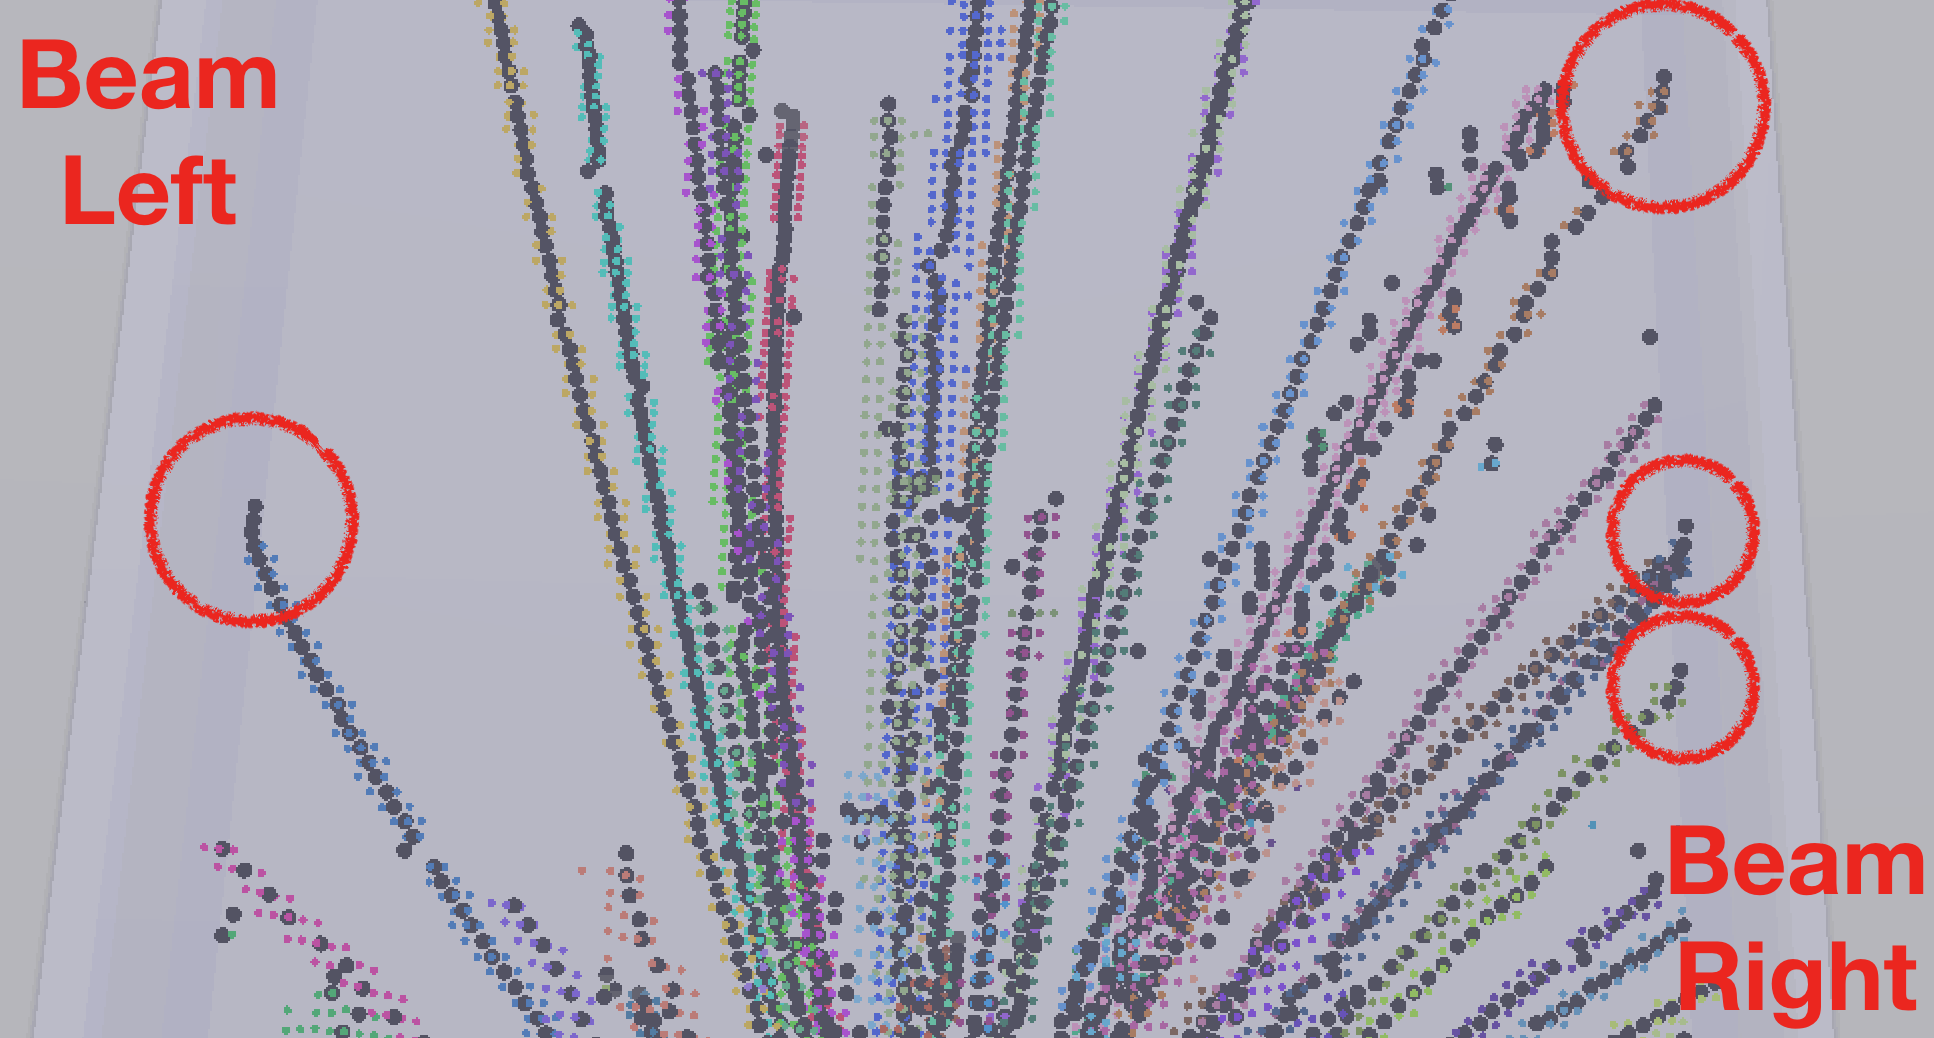
\includegraphics[width=\linewidth]{clusterLR.png} 
        \caption{Top view of the tracks showing the edge effect on the left and right sides of the TPC.} 	   \label{fig:clusterLR}
    \end{subfigure}
    \hfill
    \begin{subfigure}[t]{0.45\textwidth}
        \centering
        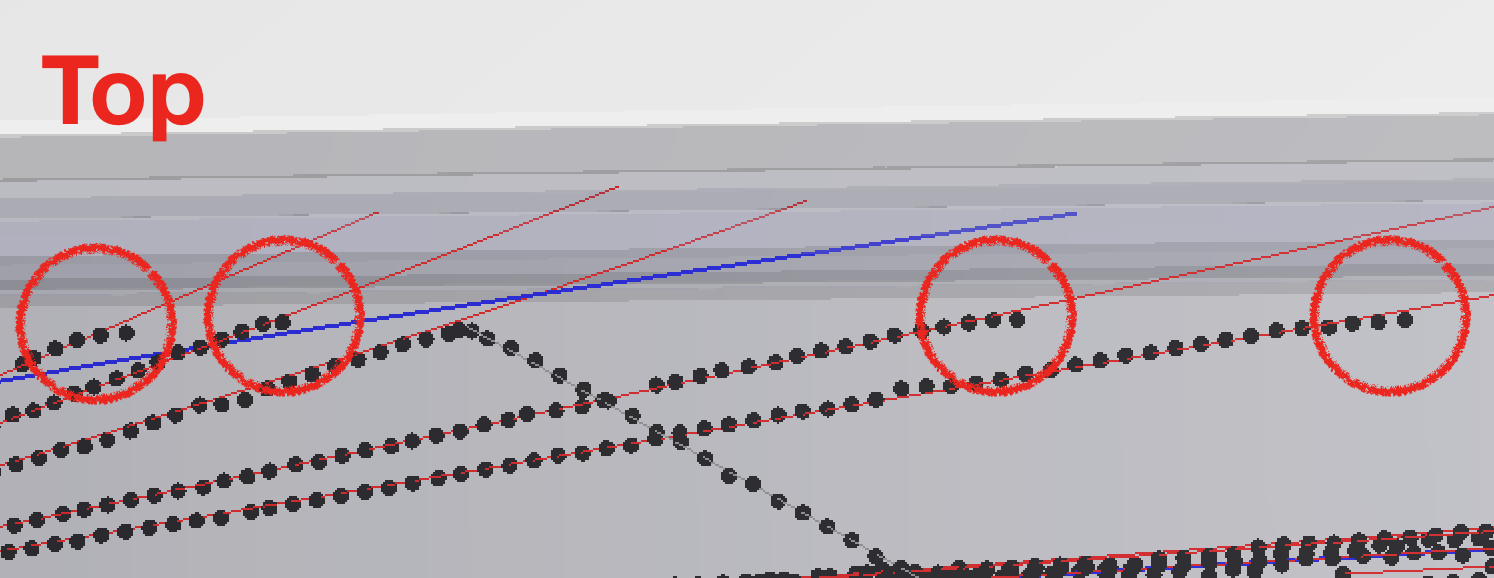
\includegraphics[width=\linewidth]{clusterTop.png} 
        \caption{Side view of the TPC showing the edge effect near the top.} \label{fig:clusterTop}
    \end{subfigure}
    
    \begin{subfigure}[t]{0.45\textwidth}
        \centering
        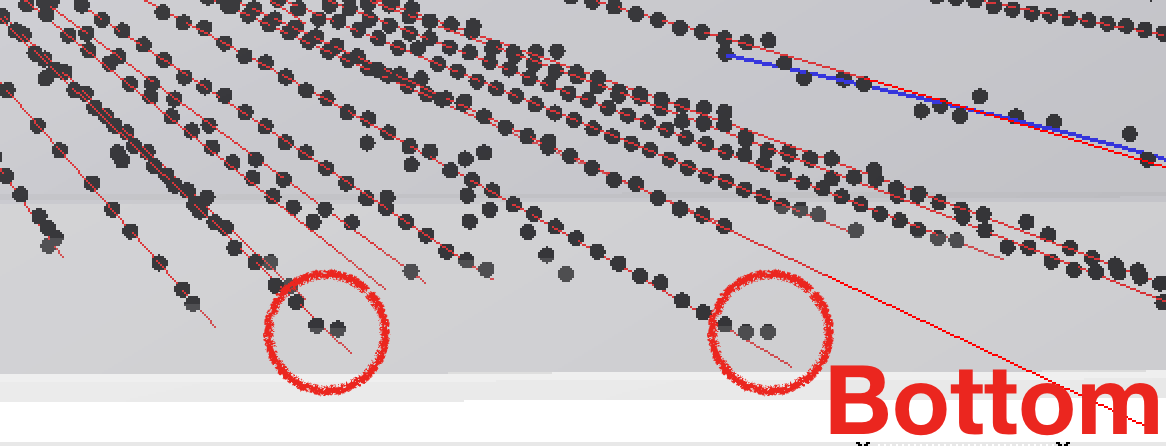
\includegraphics[width=\linewidth]{clusterBottom.png} 
        \caption{Side view of the TPC showing the edge effect near the bottom.} \label{fig:clusterBottom}
    \end{subfigure}
\caption{Example showing the edge effect has on the cluster positions near the extreme edges of the TPC volume. }    
\label{fig:edge}
\end{figure}

Near the edges of the detection volume, the clusters of tracks significantly deviate from the trend of the fitted track as seen in different view of the reconstructed clusters in Figure~\ref{fig:edge}.  This happens because the last pads on the edges of the pad-plane have no neighboring pads containing charge, and therefore the last pad represents the last known position of the collected charge. In this case the cluster position is biased towards the inside of the TPC. This also occurs for the first and last time bucket in the vertical direction. While the number of affected clusters is small, compared with the total number in the track, the deviation at the end of the track is enough cause issues in the momentum reconstruction. Simple cuts were taken to graphically remove these clusters around the left,right, top, and bottom of the TPC. The hits that were cut out satisfied the following conditions, 

\begin{equation*}
  |x|\geq420~\mathrm{mm},\quad y\leq-522+\mathrm{y_o}~\mathrm{mm},
  \quad\mathrm{and}\quad y\geq-64+\mathrm{(Hit\ Shift)}~\mathrm{mm}.
\label{eq:hitshift}
\end{equation*}



\section{High Density Cut}


\begin{figure}[!htb]

     \centering
     \begin{subfigure}[b]{0.49\textwidth}
         \centering
         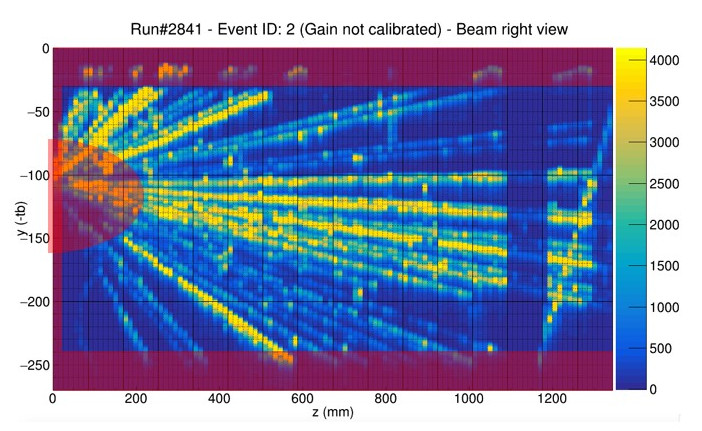
\includegraphics[width=\textwidth]{sideviewHighDenCut.jpg}
         \caption{Side view.}
         \label{fig:sideHigh}
     \end{subfigure}
     \hfill
     \begin{subfigure}[b]{0.49\textwidth}
         \centering
         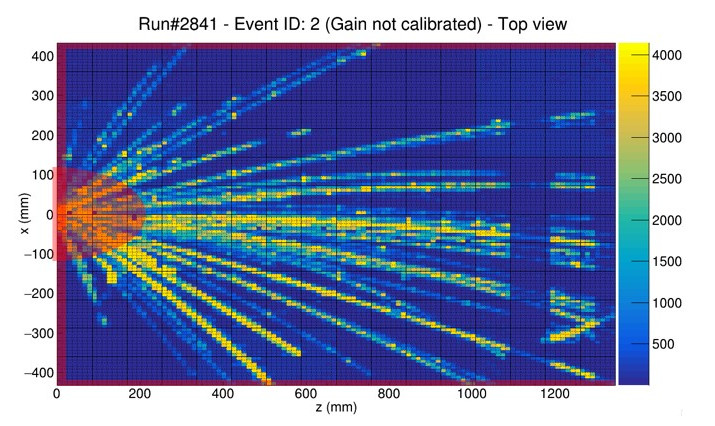
\includegraphics[width=\textwidth]{topviewHighDenCut.jpg}
         \caption{Top view.}
         \label{fig:topHigh}
     \end{subfigure}
        \label{fig:highcut}
        \caption{Views showing the high density and edge cuts.}
        \label{fig:elipsecut}
\end{figure}

The track multiplicity in the TPC ranges from 20-80 tracks. Since all the tracks originate from a common vertex, the density of tracks near the target region is very high. In this region the separation between tracks is too small for the software to correctly determine which clusters belong to which tracks, making the information useless or even incorrect. Also, the information provided by extra vertex point from external BDC tracking described in \ref{sec:bdc}, provides all the information about the vertex location. The bad quality of hit information near the target region only hurt in the tracking and PID of a track. Hits lying within an semi-ellipsoidal cut around the target are removed from the software and not included in the track and momentum reconstruction. Figure~\ref{fig:elipsecut} shows the extent of the ellipsoidal cut in the high density region, along with the edge cuts as shaded red regions in both views of the TPC. 

\section{Beam angle selection}
\label{sec:beamangle}
The incoming secondary beam is deflected by the magnetic field and impinges on the target at some angle. From the BDC tracking information, the beam is projected as a straight line right up until entering the magnet.  The beam is then propagated through the magnetic field using a Runge-Kutta integration until reaching the target position \cite{jon}. The beam angle on target can be categorized by two angles $\theta_{a_{proj}}$ and $\theta_{b_{proj}}$ where $p_x$, $p_y$, and $p_z$ are the components of beam momentum vector:

%define angles 
%define selection

\begin{equation}
  \theta_\mathrm{a,proj}=\tan^{-1}\frac{p_x}{p_z},\quad
  \theta_\mathrm{b,proj}=\tan^{-1}\frac{p_y}{p_z}.
  \label{beamAngle}
\end{equation}





\begin{table}[!htb]
  \begin{center}
    \begin{tabular}{ccccc}
      \hline 
      System & $\mu_{\theta_\mathrm{a,proj}}$ &
      $\sigma_{\theta_\mathrm{a,proj}}$ & $\mu_{\theta_\mathrm{b,proj}}$ &
      $\sigma_{\theta_\mathrm{b,proj}}$ \\
      \hline\hline 
      $\tin{132}{124}$ & 0.61 & 2.94 & -44.18 & 1.96 \\
    %  $\tin{112}{124}$ & -0.41 & 1.58 & -53.52 & 0.90 \\
      $\tin{108}{112}$ & -0.42 & 1.95 & -55.17 & 0.97 \\
      \hline
    \end{tabular}
    \caption{2D Gaussian fit parameters for $^{132}$Sn, $^{112}$Sn and
      $^{108}$Sn beam angle cuts. \label{beamAngleParameters}}
  \end{center}
\end{table}

\begin{figure}[!htb]
    \centering
    \begin{subfigure}[t]{0.45\textwidth}
        \centering
        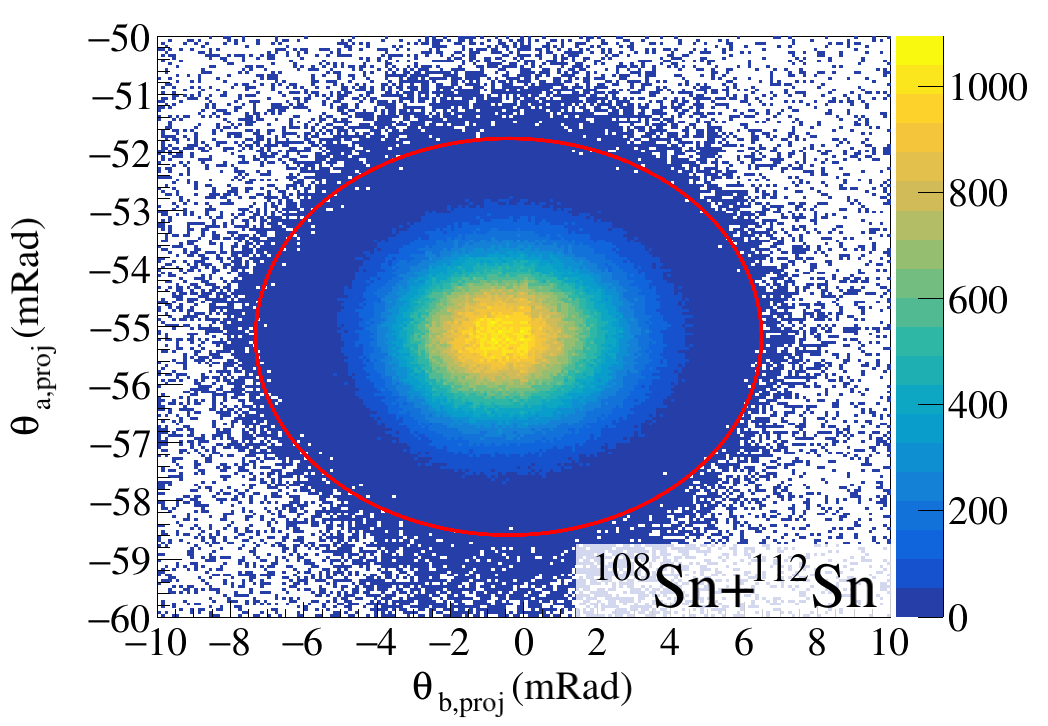
\includegraphics[width=\linewidth]{beamAngle-Sn108.png} 
        \caption{Beam angle of the $\tin{108}{124}$ system} \label{fig:beamangle108}
    \end{subfigure}
    \hfill
    \begin{subfigure}[t]{0.45\textwidth}
        \centering
        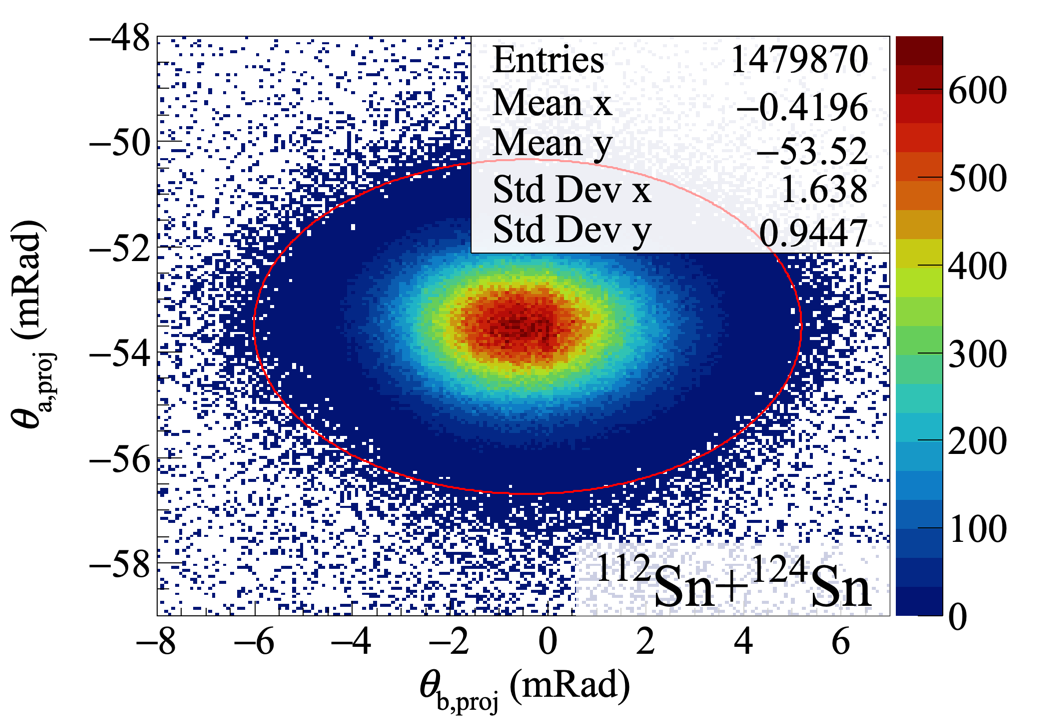
\includegraphics[width=\linewidth]{beamAngle-Sn112.png} 
        \caption{Beam angle of the $\tin{112}{124}$ system} \label{fig:beamangle112}
    \end{subfigure}
    
    \begin{subfigure}[t]{0.45\textwidth}
        \centering
        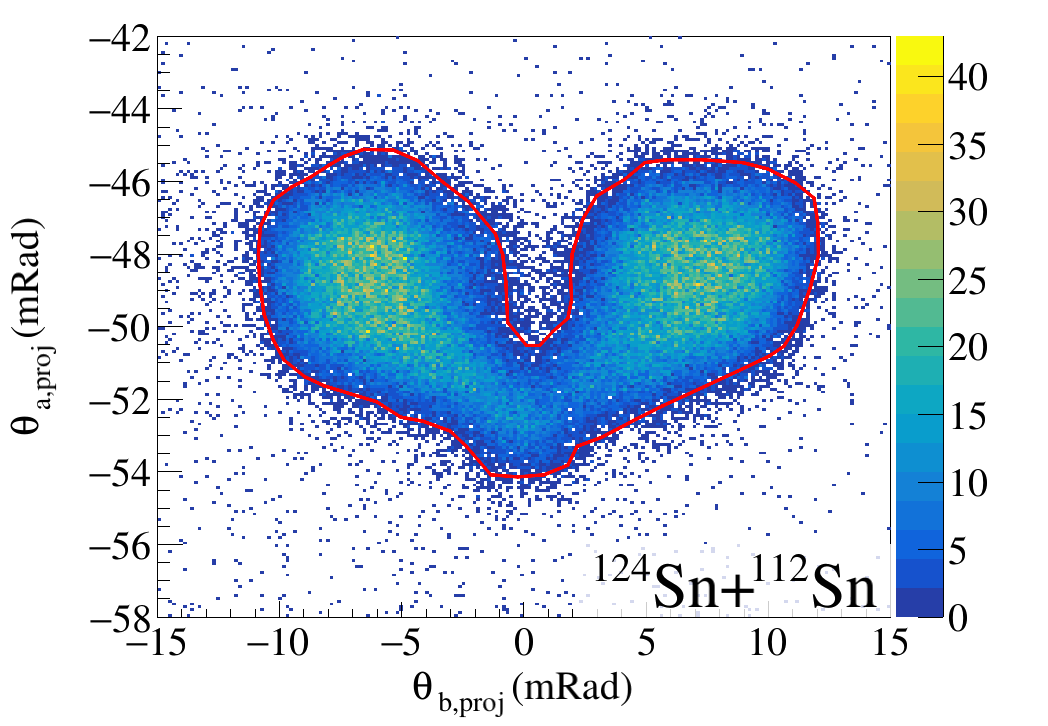
\includegraphics[width=\linewidth]{beamAngle-Sn124.png} 
        \caption{Beam angle of the $\tin{124}{112}$ system} \label{fig:beamangle124}
    \end{subfigure}
    \hfill
    \begin{subfigure}[t]{0.45\textwidth}
        \centering
        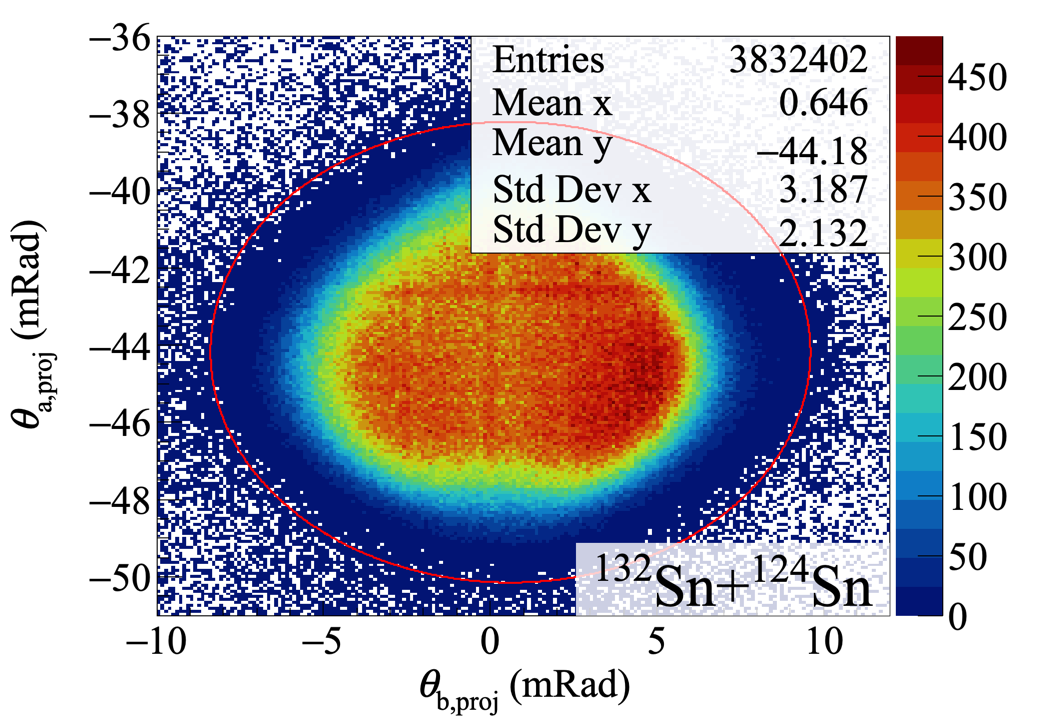
\includegraphics[width=\linewidth]{beamAngle-Sn132.png} 
        \caption{Beam angle of the $\tin{132}{124}$ system} \label{fig:beamangle132}
    \end{subfigure}
\caption{Beam angle at the face of the target in the TPC for all 4 systems.}
\label{fig:beamangle}
\end{figure}


Figure~\ref{fig:beamangle} shows the distribution of beam angles for ${}^{132}$Sn and ${}^{108}$Sn systems. Graphical cuts represented by the red lines where events lying in the cuts represent beams that were reconstructed correctly by the beam tracking software outlined in \cite{jon}. This helped to eliminate some of the poorly reconstructed beam events. The angle rotation becomes important in the discussion of transforming back to the center-of-mass system as will be discussed in Section~\ref{sec:pionSpectra}.



\section{Vertex Cut}
\label{sec:vertexcut}

\begin{figure}[!htb]
\centering
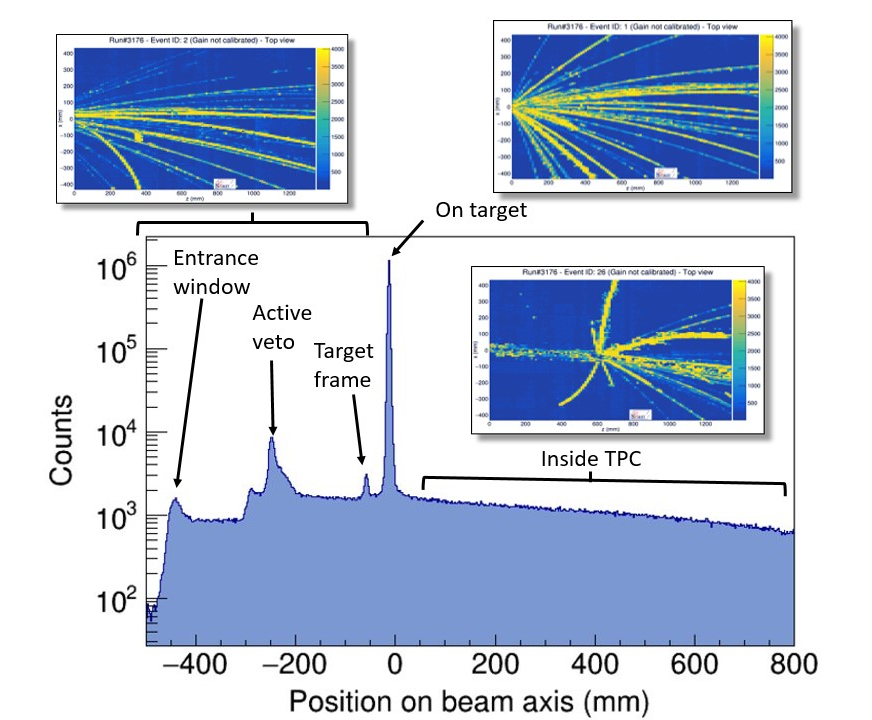
\includegraphics[scale =.5]{vertexDistribution.png}
\caption{Projection of the vertex onto the z-axis.}
\label{fig:overviewVertex}
\end{figure}


\begin{figure}[!htb]
\centering
    \begin{subfigure}[t]{\textwidth}
        \centering
        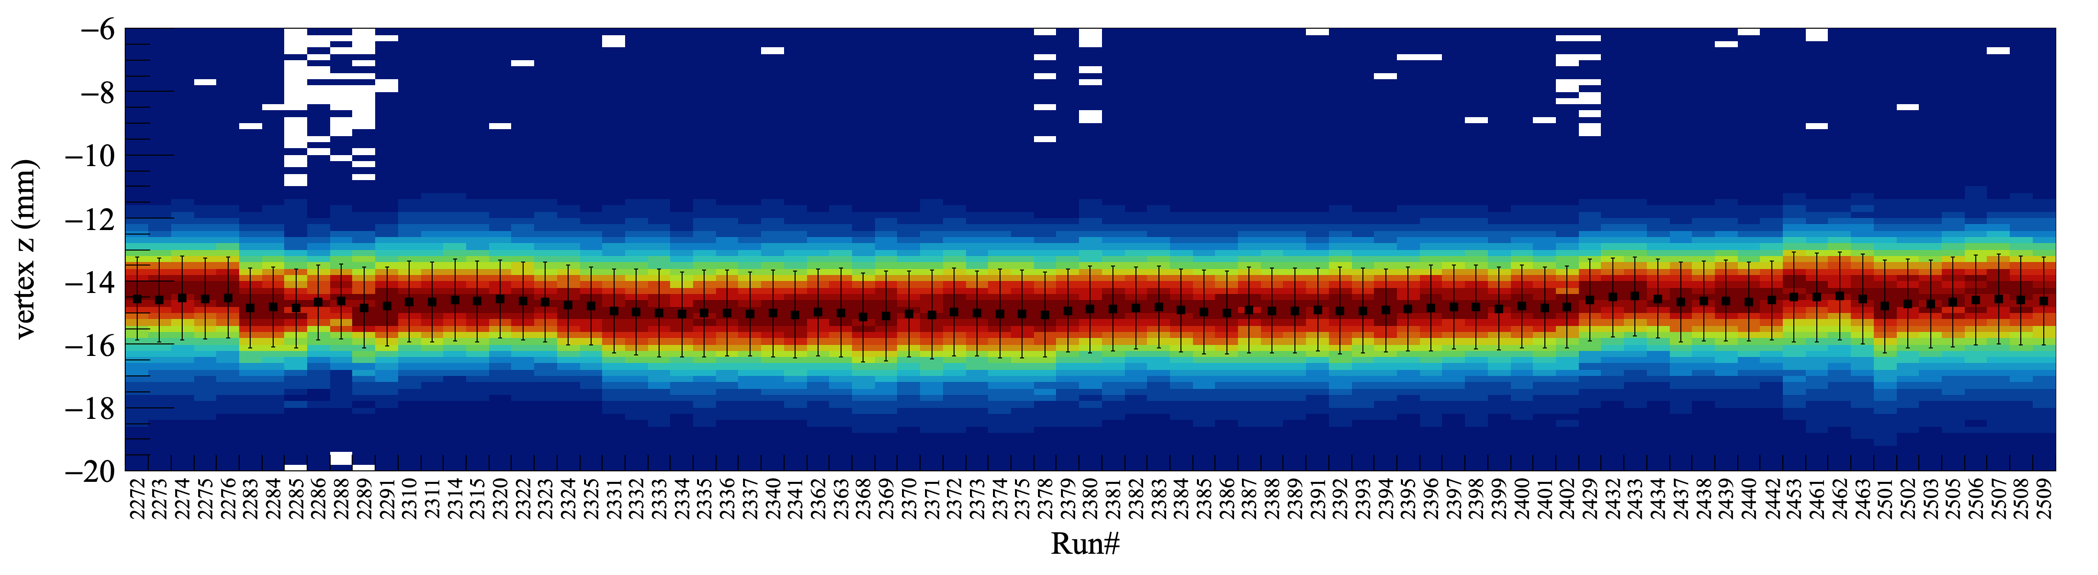
\includegraphics[width=\textwidth]{vertex-Sn108.png} 
        \caption{$\tin{108}{124}$ system.} \label{fig:vertex108}
    \end{subfigure}
    \hfill
    \begin{subfigure}[t]{\textwidth}
        \centering
        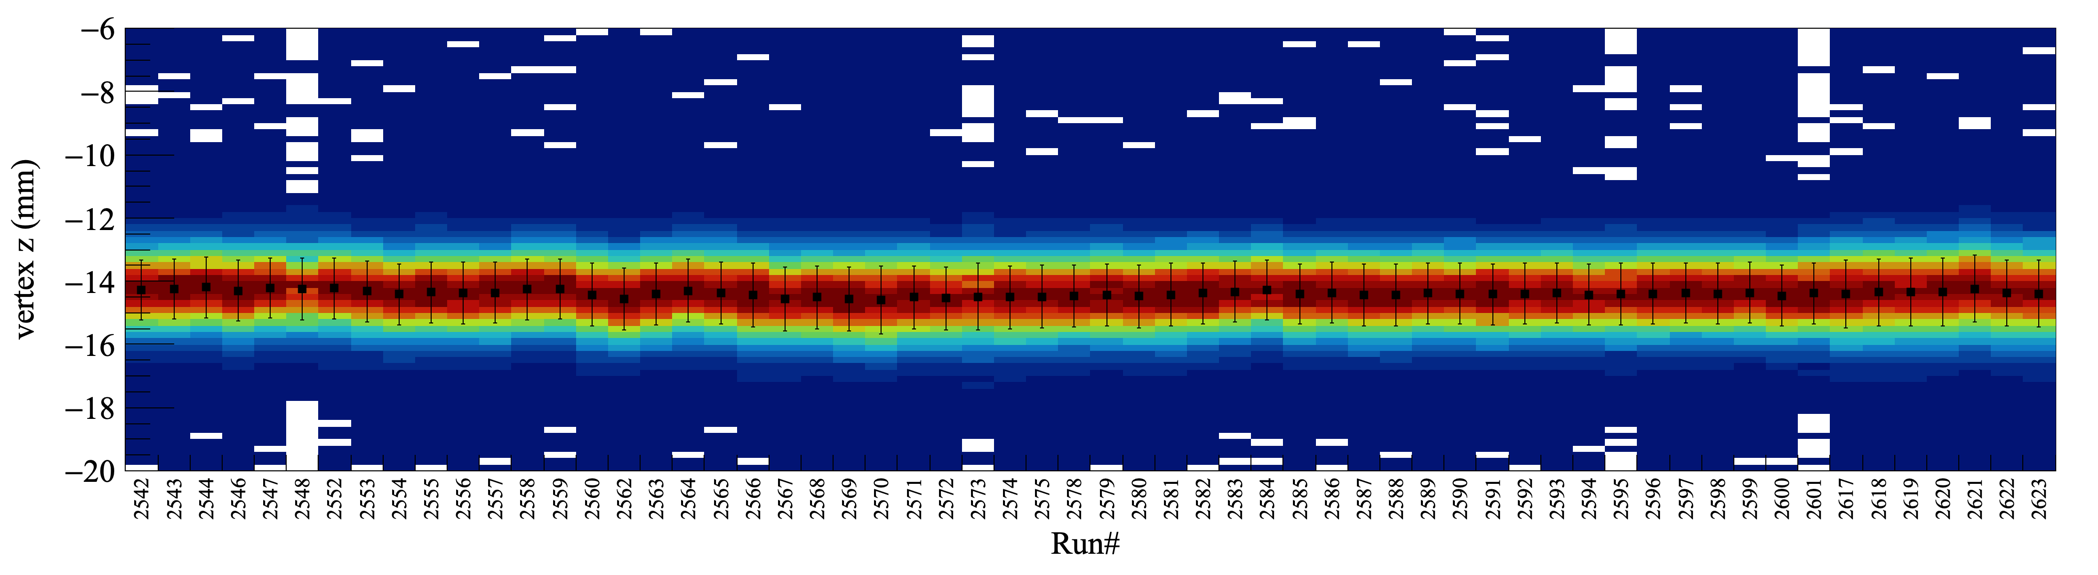
\includegraphics[width=\textwidth]{vertex-Sn112.png} 
        \caption{$\tin{112}{124}$ system.} \label{fig:vertex112}
    \end{subfigure}
    
    \begin{subfigure}[t]{\textwidth}
        \centering
        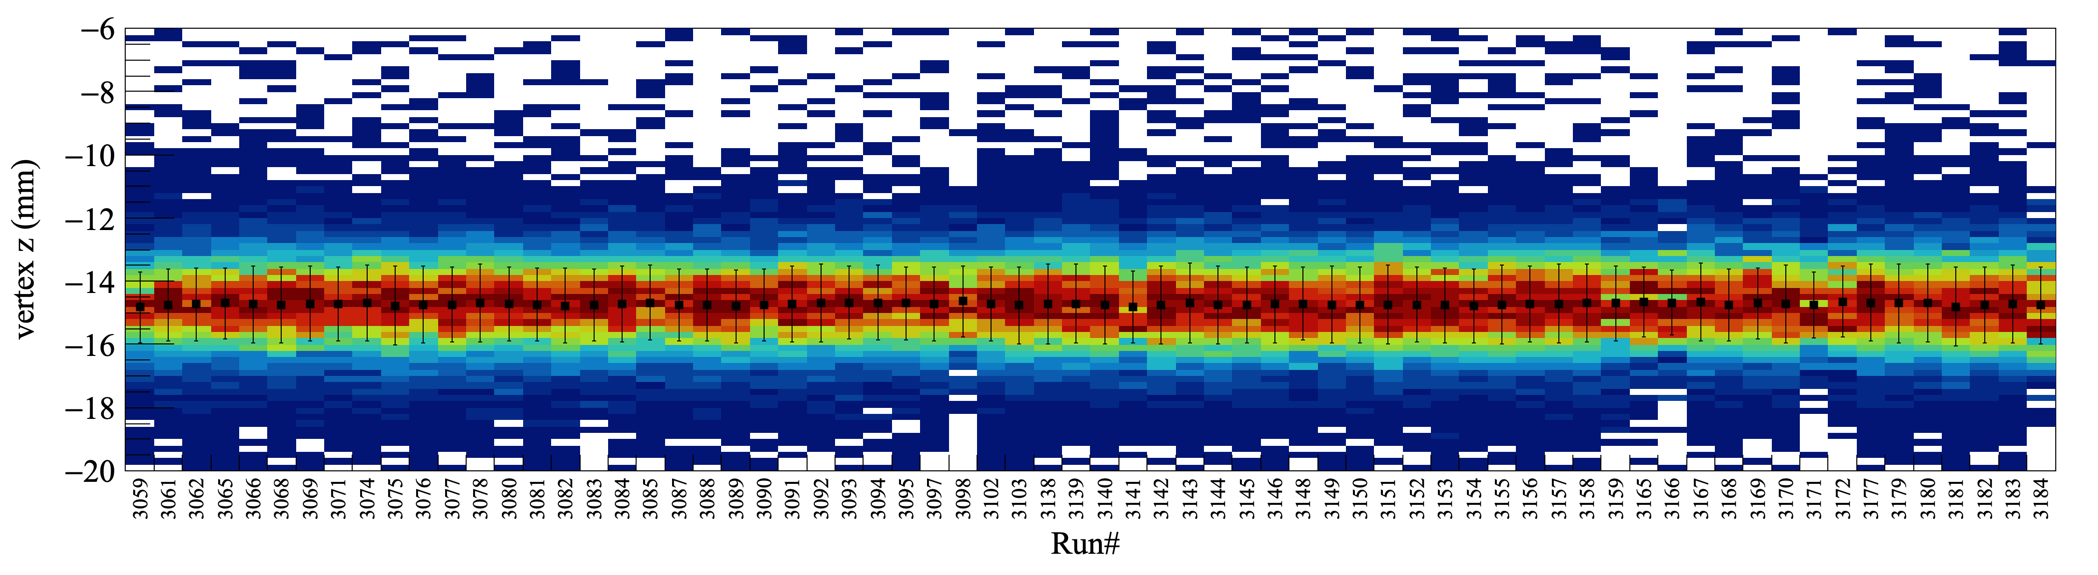
\includegraphics[width=\textwidth]{vertex-Sn124.png} 
        \caption{$\tin{124}{112}$ system.} \label{fig:vertex124}
    \end{subfigure}
    \hfill
    \begin{subfigure}[t]{\textwidth}
        \centering
        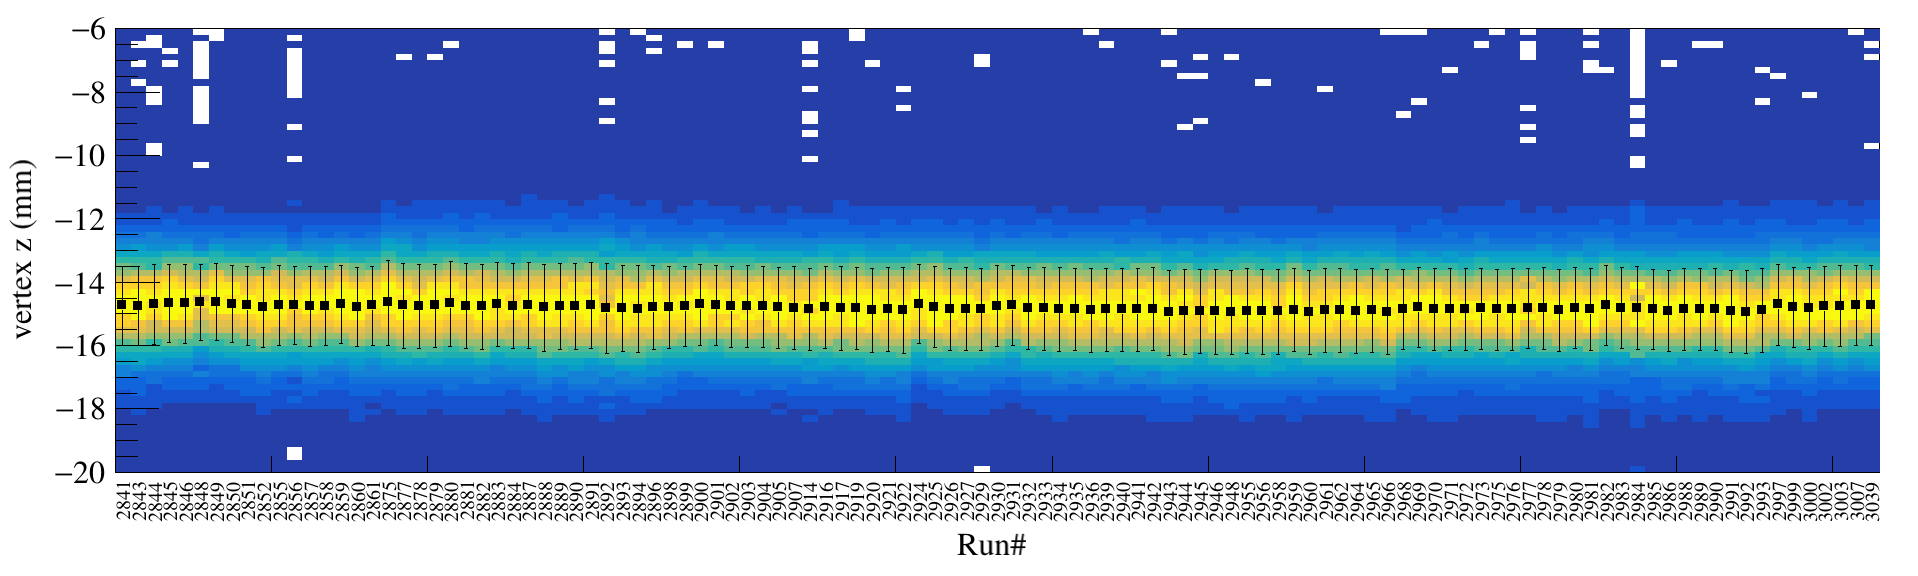
\includegraphics[width=\textwidth]{vertex-Sn132.png} 
        \caption{$\tin{132}{124}$ system.} \label{fig:vertex132}
    \end{subfigure}
\caption{Vertex distributions, around the target region, of all experimental runs for each secondary beam system. }
\label{fig:vertexdist}
\end{figure}

The vertex information of an event, described in \ref{sec:vertex}, is estimated from reconstructing the tracks of an event to one common point. The secondary beam encounters several solid and gaseous materials along the beam line where a nuclear reaction can occur. Figure~\ref{fig:overviewVertex} shows the z-component of the reconstructed vertex for all events in the ${}^{132}$Sn system. Several peaks are seen in the spectrum which correspond to several dense materials in the beam line such as the entrance windows, target frame, Active Veto, with the largest peak representing the target. Collisions also happen with the detector gas inside the TPC volume where the gas acts as a target. To ensure that the secondary beam is really on the target of choice we perform a vertex cut around where we believe the vertex location of the target to be.
 
 The target position was physically expected to be \SI{-13.2}{\milli\metre} in the TPC coordinate frame. The z-component of all runs in each beam type are plotted around the the target region in Figure~\ref{fig:vertexdist}. The mean position of the vertex from the reconstructed data is around \SI{-14.76}{\milli\metre} which is about \SI{1.6}{\milli\metre} off from the expected target position. The mean position for each system is listed in Table~\ref{tb:vertexresol}. Since the target thickness was less than \SI{1}{\milli\metre} for all targets, we can assume the thickness of the target has a minimal effect on the vertex resolution of the TPC. Therefore the measured width of the vertex distribution can be interpreted directly as the vertex resolution of the TPC. The extracted vertex resolutions of each system are summarized in Table~\ref{tb:vertexresol}, with an average vertex resolution of \SI{1.2}{\centi\metre}. The difference between the measured and actual target location is 10 times smaller than the intrinsic vertex resolution of the detector and is an insignificant difference.  



\begin{table*}\centering
\ra{1.3}
\begin{tabular}{@{}rrr@{}}\toprule
\multicolumn{3}{c}{Vertex Resolution}\\
\cmidrule{1-3}
System & Mean (cm) & Sigma (cm) \\
\midrule
$\tin{132}{124}$ & -14.79  & 1.2 \\
$\tin{124}{112}$ & -14.71  & 1.1 \\
$\tin{112}{124}$ & -14.78  & 1.2 \\
$\tin{108}{112}$ & -14.75  & 1.3 \\ 
\bottomrule
\end{tabular}
\caption{Summary of the mean vertex location for the target position in all systems and the measured vertex resolution.}
\label{tb:vertexresol}
\end{table*}


\clearpage

\section{Impact Parameter Selection}
\label{sec:impact}

\begin{figure}[htb]
\centering
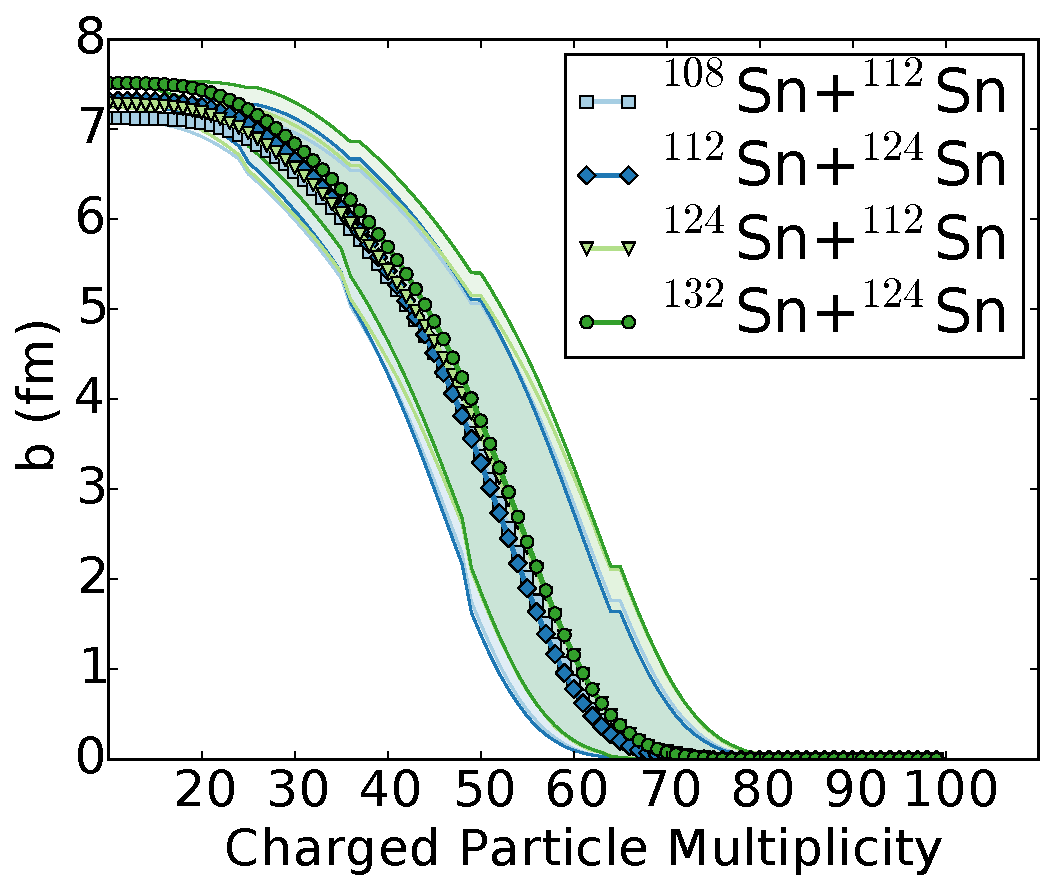
\includegraphics[scale=.5]{error_b_full.pdf}
\caption{Estimate of the impact parameter from the track multiplicity.}
\label{fig:impactPar}
\end{figure}

The impact parameter is a theoretical quantity defined as the distance between two centers of colliding nuclei. Though there is no way to directly measure the impact parameter in an experiment, the track multiplicity is indirectly related to the estimated impact parameter of a collision \cite{impactpar}. As discussed in Section \ref{sec:kyoto}, the Kyoto multiplicity array was used to experimentally trigger on central nuclear collision events. This is under the assumption that number of charged particles produced in collision is related to the overlap region of the two nuclei. This is best described by a spectator-participant model of nuclear collisions, where a large fraction of the participating nucleons in the overlap region of the two colliding nuclei fragment into individual and clusters of nucleons. In the case where the impact parameter is zero, all the nucleons in both nuclei participate, were as larger impact parameters -- more peripheral collisions -- less nucleons participate. 


%Certainly the Kyoto array introduces a bias in our measurement of the multiplicity of all the events. At low track multiplicities, the orientation of the event starts to play a major role. Theoretically the orientation of the event (the reaction plane) is random, but due to the fact that we only measure the multiplicity on the sides of the TPC, we are preferentially triggering on events with reaction planes that emit particles in these directions. Therefore events with low track multiplicity (therefore more peripheral), that emit preferentially up and down in the TPC will not be triggered on. This becomes less of an issue as even in mid-peripheral collisions were the number of particles emitted becomes much greater than the Kyoto multiplicity selection

The geometric cross section $\sigma$ can be described as, 

\begin{equation}
\sigma = \pi \cdot b^2,
\label{eq:crossSect}
\end{equation}

where $b$ is the impact parameter of the collision.  If the track multiplicity of an event $N_C$ is monotonically related to the cross section, the impact parameter can be written as a reduced impact parameter $\hat{b}$ as,
\begin{equation}
\hat{b} =  \frac{b}{b_{max}} = \int^{\infty}_{N_C} \frac{dP(N_C)}{dN_C} dN_C,
\end{equation}

where $b_{\mathrm{max}}$ represents the maximum impact parameter detected by the TPC, $b$ is the impact parameter of the vent,  and $dP(N_C/dN_C$ is the normalized multiplicity distribution \cite{reducedimpact}. The reduced impact parameter ranges from $\hat{b}=0$ for the most central collisions and to $\hat{b}=1$ for the most peripheral. A  detailed analysis was performed, determining the maximum cross section $\sigma_{max}$, for each system, in which $b_{\mathrm{max} = \sqrt{\sigma_{max}/\pi}}$. The detailed analysis is given in \cite{jon}. Figure~\ref{fig:impactPar} shows the estimated impact parameter for a given track multiplicity with the estimated error bands for each system. 

In the $\tin{132}{124}$ system the multiplicity cut was $N_C > 50$ corresponding to $\hat{b} = 0.4$ and $b = \SI{3.1}{\femto\metre}$. For the $\tin{108}{112}$ system the multiplicity cut was $N_C > 49$ corresponding to $\hat{b} = 0.4$ and $b = \SI{3.1}{\femto\metre}$. These values were averaged over the multiplicity distribution as,

\begin{equation}
 \overline{X} = \int_{N_C}^{\infty} X\frac{dP(N_C)}{dN_C} dN_C
\end{equation}

where X can be the variables $b$, $\hat{b}$. In the $\tin{132}{124}$ system the average $\overline{\hat{b}} = \num{.1(1)}$ and $\overline{b} = \SI{3}{\femto\metre}$. In the $\tin{108}{112}$ system the average $\overline{\hat{b}} = .1$ and $\overline{b} = \SI{3}{\femto\metre}$. These quantities are useful when comparing to theory. 

\section{Track Quality Cuts}
\label{sec:qualitycut}
%graphic showing distance to vertex, number of clusters
%number of cluster cut
%distance to vertex
In this section we will discuss cuts which address the quality of the reconstructed track, in the following we will simply refer this as the \emph{track quality}. Assuming tracks are mostly continuous in clusters, i.e. only randomly missing a few clusters, the number of clusters is directly related to the momentum resolution of a track. Tracks with more clusters correspond to better PID and momentum resolution. Upward-going and downward-going tracks, at larger values of $\theta_{Lab}$ are limited by the vertical space of the TPC. In these regions the track length is short and there are few clusters which are reconstructed. This leads to the low efficiency in these regions as discussed earlier in Sec.~\ref{sec:efficiency}. A cut where tracks with the number of clusters $N_{cl} > 20$ are considered quality tracks. Later in Section~\ref{sec:cutvar} the exact choice of the number 20 is discussed in more detail.

\begin{figure}[!htb]
\centering
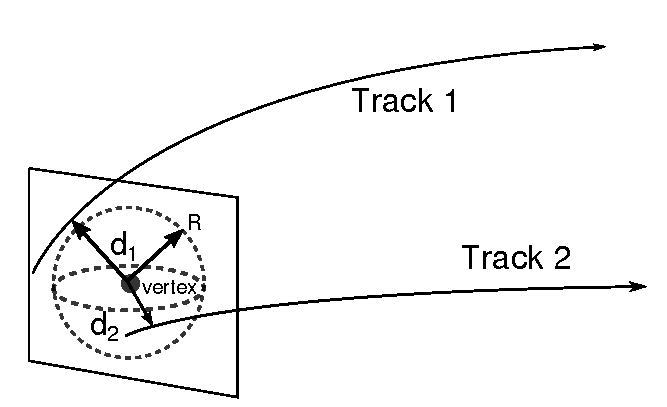
\includegraphics[scale=1.]{distancetovertex.pdf}
\label{fig:poca}
\caption{Example diagram of the Distance of Closest Approach (DOCA) cut for tracks.}
\end{figure}

For very long tracks, such as low momentum pions, which can make a complete circular path in the TPC, it can happen that the software incorrectly identifies the track as several separate tracks. This can happen due to discontinuities in the track due to missing hits from low energy loss, shadowing due to saturation, or possibly the software algorithm itself. Including all of the tracks would be counting the track several times over, and would lead to incorrect particle yields. The software can also occasionally associate random disassociated clusters and construct a false track, or a so called \emph{ghost track}. These type of tracks contribute to the background in the PID. In both of these situations the track origin cannot be traced back to anywhere near the vertex of the event, and the distance-Of-Closest-Approach (dOCA) between the track and vertex is very large. 

To reduce the number of false tracks, a simple cut on the dOCA can be used. The vector representing the minimum distance to vertex for each track can be calculated and its corresponding magnitude. We define the distance to vertex cut as a small sphere centered around the vertex location with a some radius $R$. If the dOCA of a particular track $d_i < R$, the track is assumed to have originated from the vertex; tracks outside of the cut are thrown out of the analysis. 


\section{Angular Quality Cuts}

Since the TPC does not have spherical symmetry, there are regions of bad geometric acceptance that effect the efficiency of track reconstruction. Most notably upward and downward-going tracks will have the shortest track length and will correspond to low regions of efficiency as seen in \ref{sec:efficiency}. The relevant geometries which determine these regions are the corners of the field cage. Figure~\ref{fig:angleEffExplanation} shows a cartoon drawing of the front of the field cage were the angles of each corner is given. Since the window to the field cage was slightly higher, the upper angles are smaller than the lower angles. These angles are actually the same as the spherical $\phi$ angle, where the left and right, are most efficient regions, correspond to  $\ang{0}\substack{+24 \\ -34}$ and $\ang{180}\substack{+34 \\ -24}$.  While the exact area of zero efficiency depends on polar angle $\theta_{Lab}$, a clear cut off around these angles can be seen in Figure~\ref{fig:angleEffExplanation} in the angular distribution of the measured tracks. Here, the experimental data was fitted with a Fermi distribution to find the inflection point of where the efficiency drops off significantly. The angular cuts applied to the data is listed by particle type in Table~\ref{tb:anglecuts}. The values are very close to the simple calculation outlined previously. 


\begin{figure}[!htb]
\centering
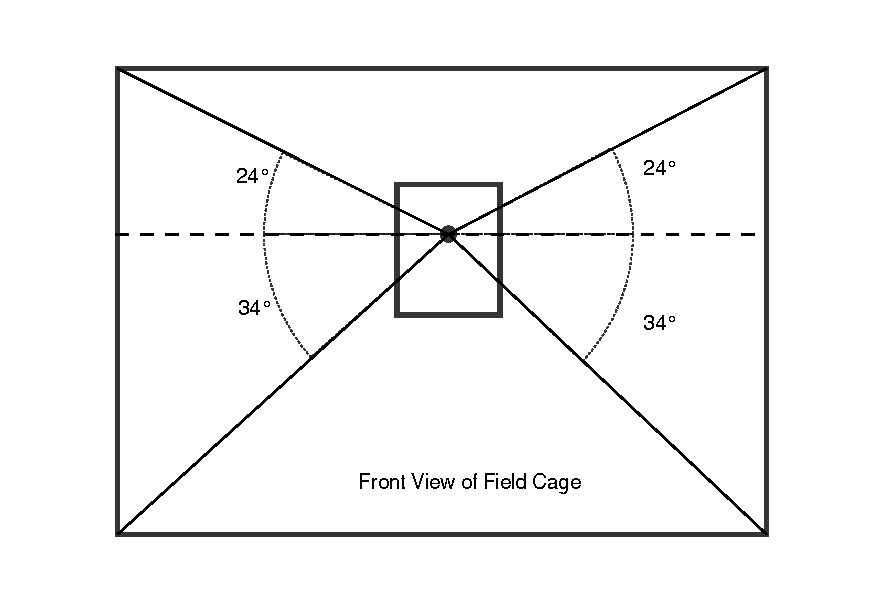
\includegraphics[scale=.75]{tpcAngle.pdf}
\caption{Rough Geometry of the TPC field cage.}
\label{fig:angleEffExplanation}
\end{figure}


\begin{figure}[!htb]
     \centering
     \begin{subfigure}[b]{0.49\textwidth}
         \centering
         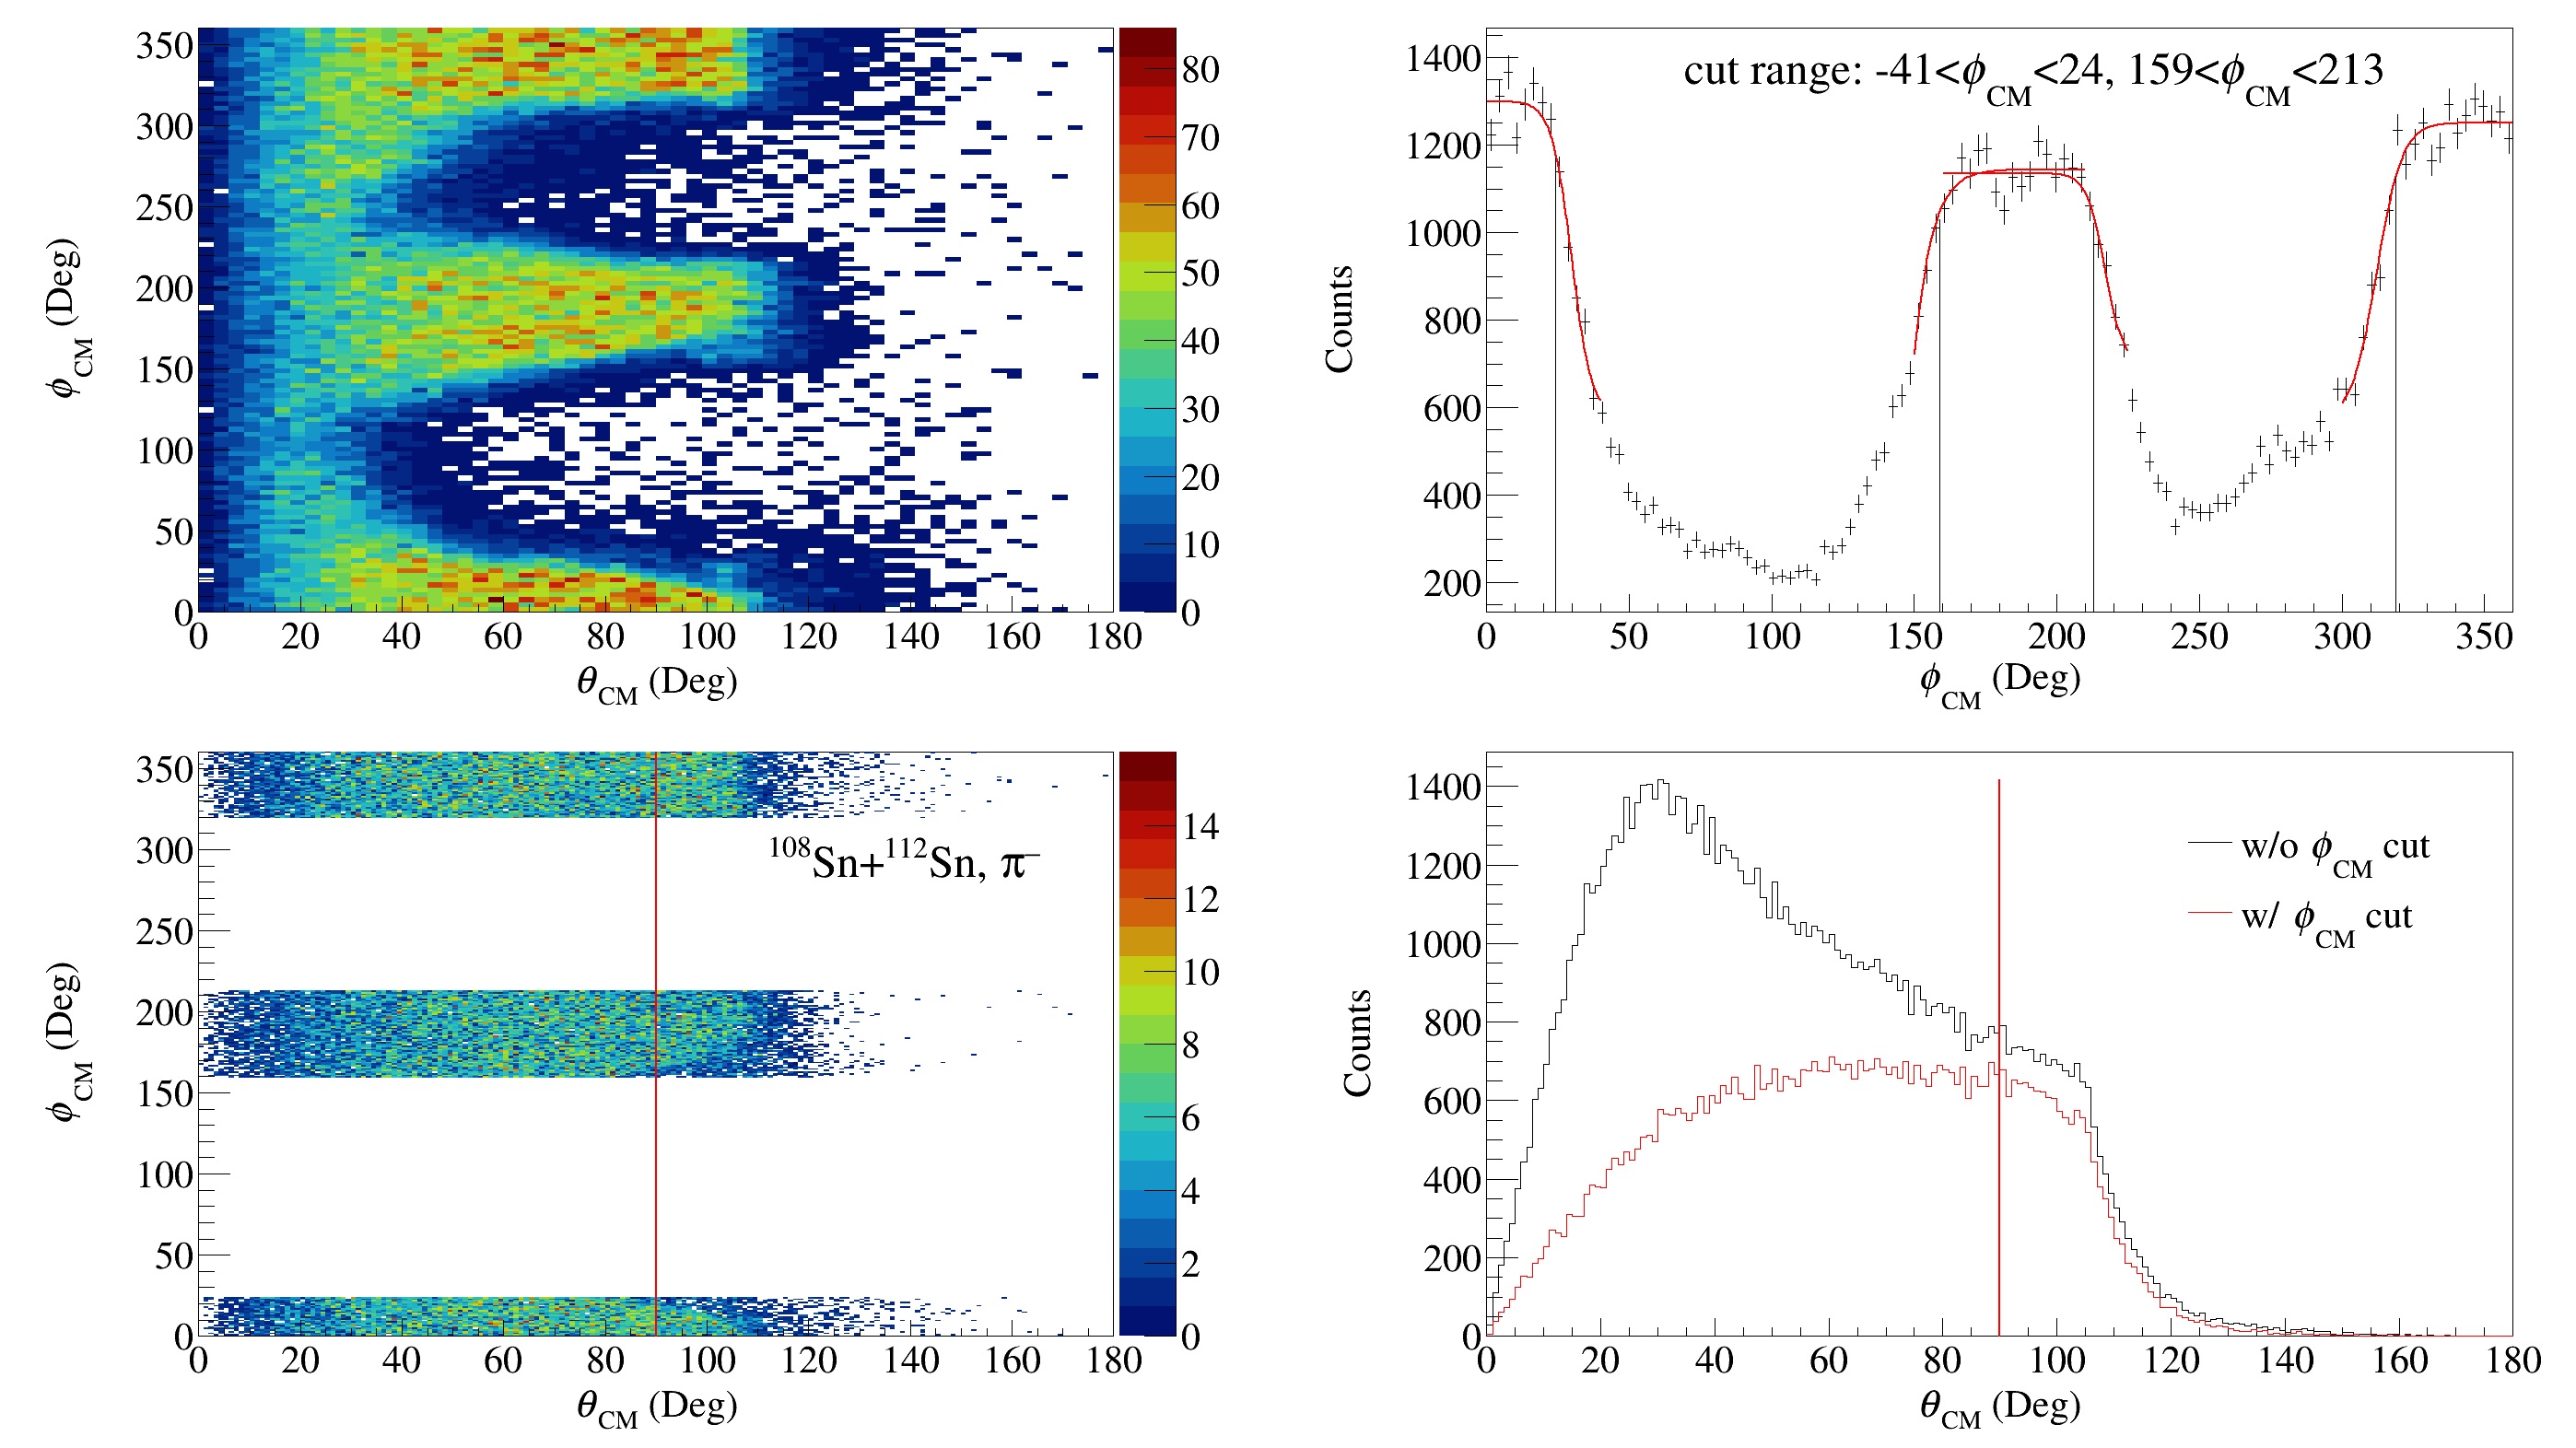
\includegraphics[width=\textwidth]{angularCut-pim-Sn108.png}
         \caption{$\pi^-$ angular cuts in the $\tin{108}{112}$ system. $\theta_{CM} < 90$ and < $\phi$ <}
         \label{fig:pim108angle}
     \end{subfigure}
     \hfill
     \begin{subfigure}[b]{0.49\textwidth}
         \centering
         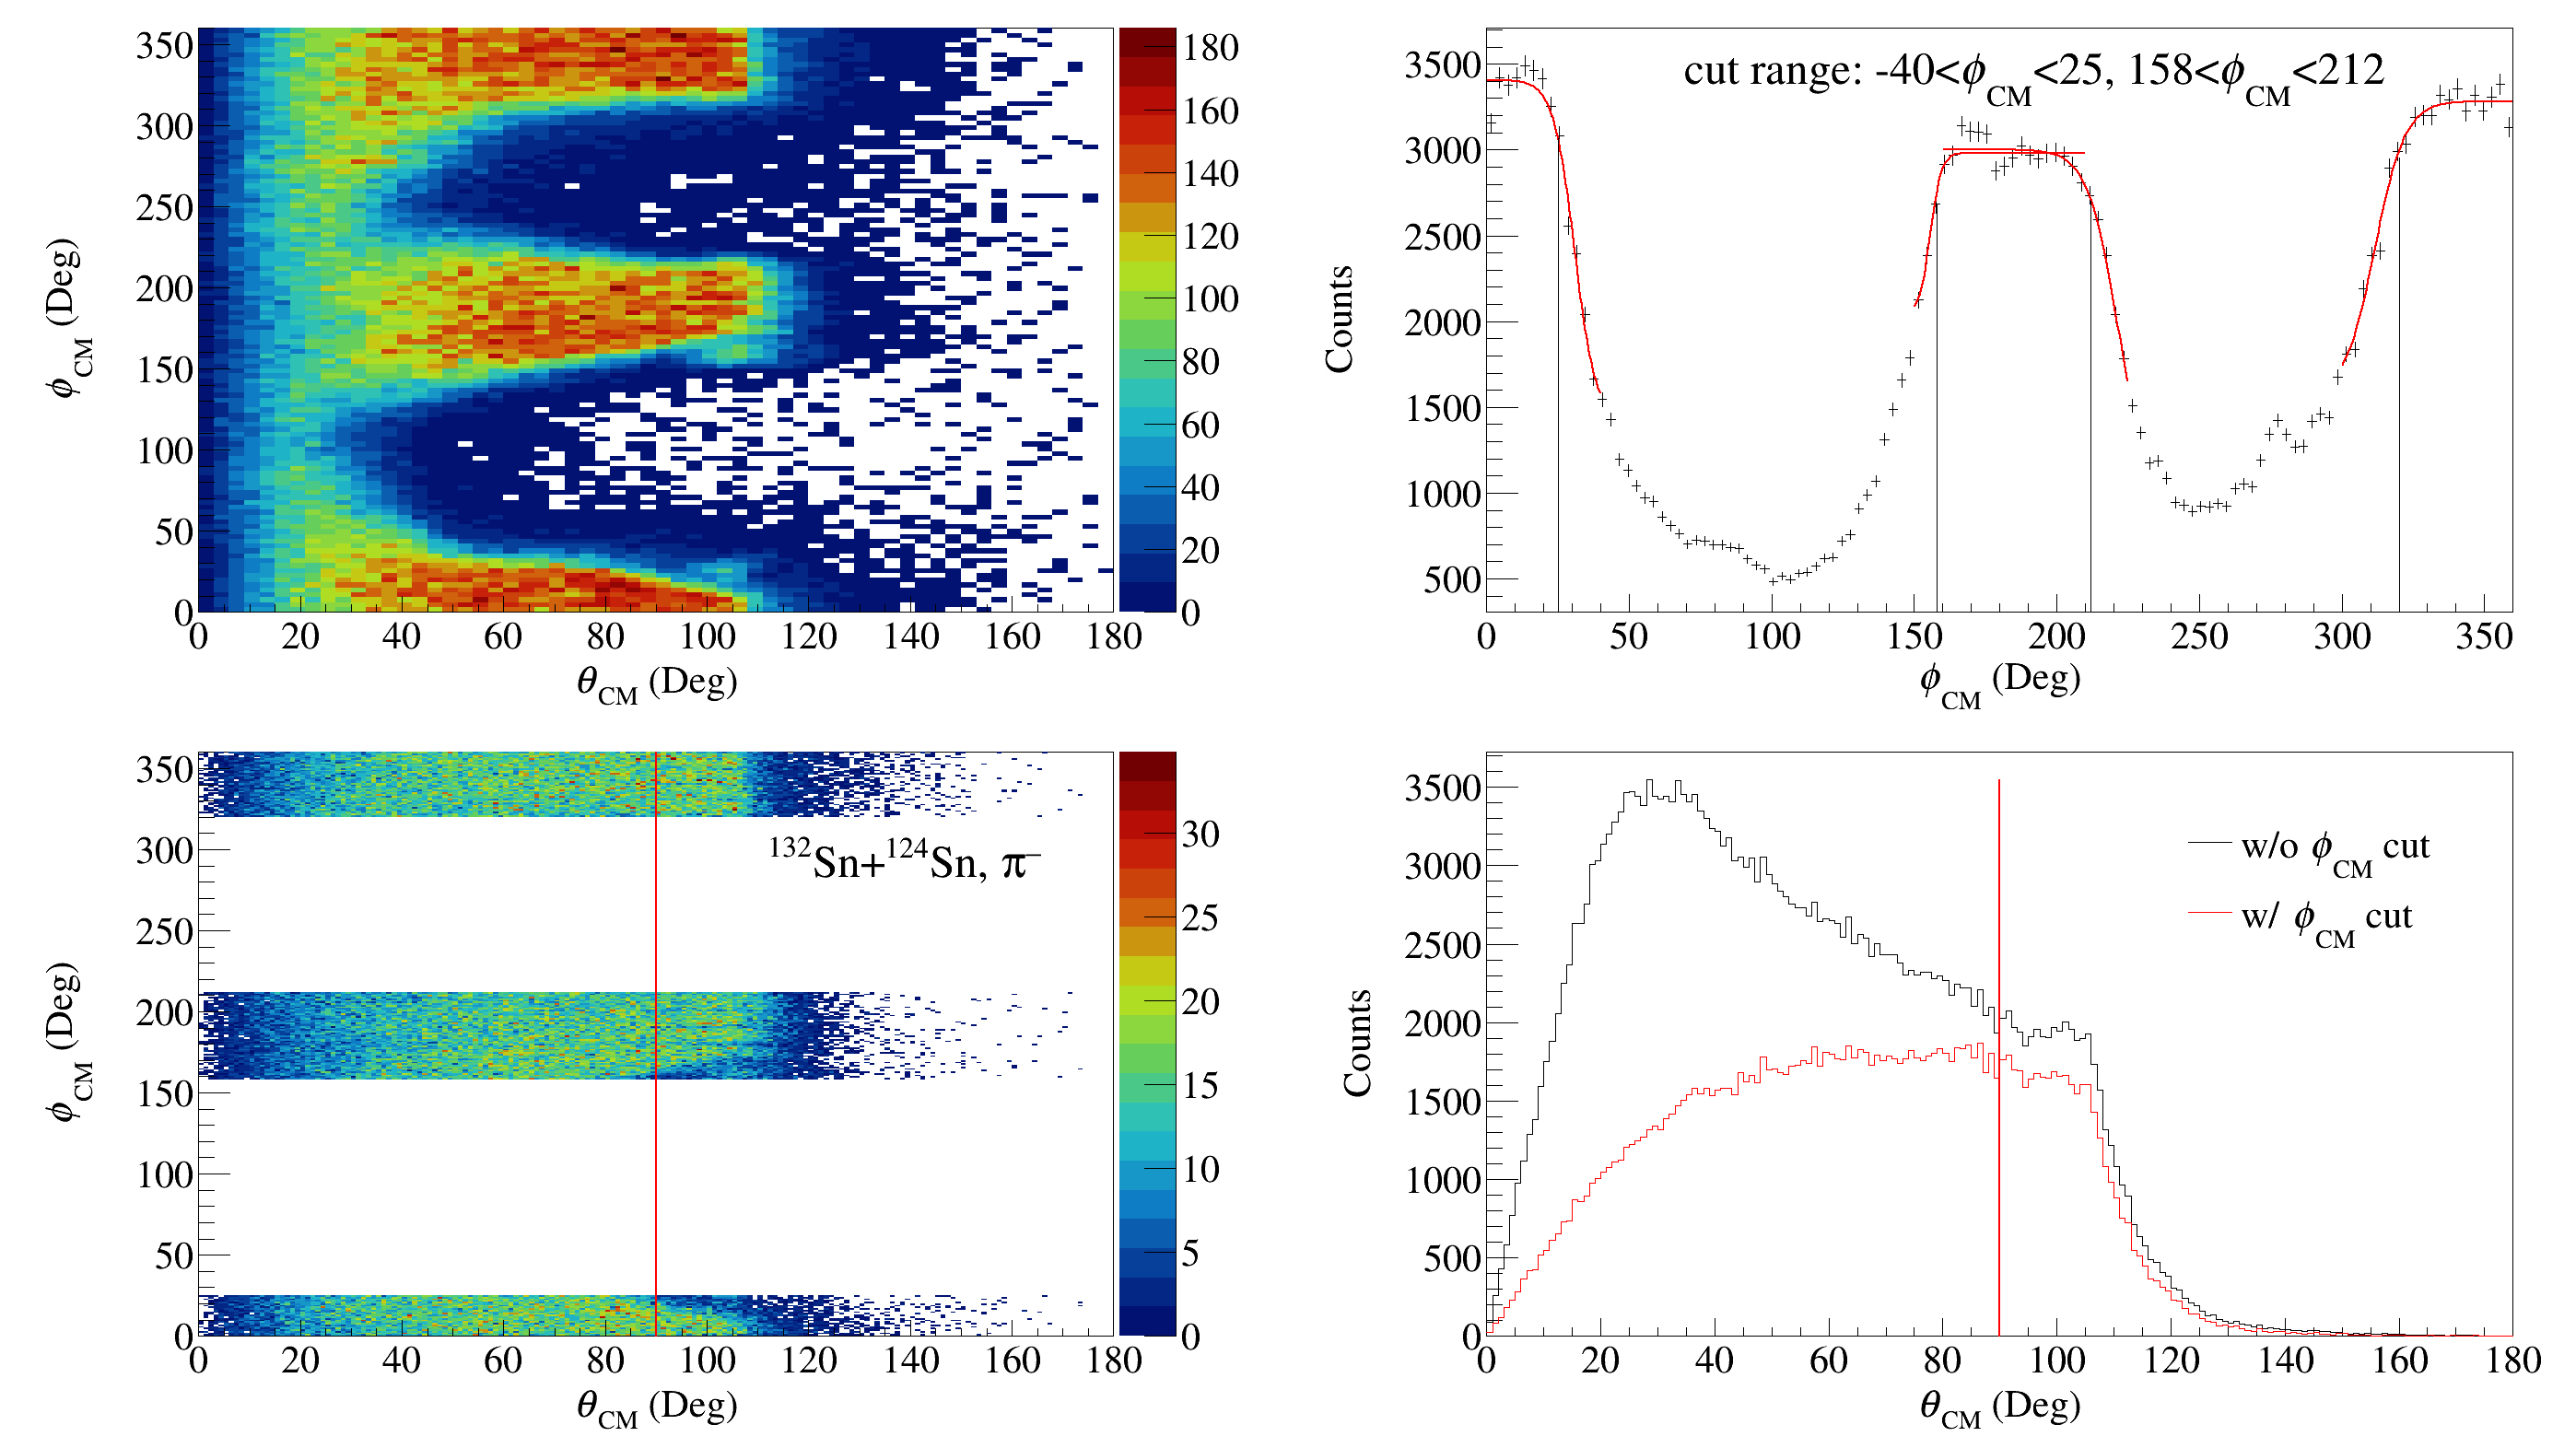
\includegraphics[width=\textwidth]{angularCut-pim-Sn132.png}
         \caption{$\pi^-$ angular cuts in the $\tin{132}{124}$ system. $\theta_{CM} < 90$ and < $\phi$ <}
         \label{fig:pim132angle}
     \end{subfigure}
        \caption{Measured $\pi^-$ angular distribution for the two spherical angles $\theta$ and $\phi$.}
        \label{fig:pim}
\end{figure}


\begin{figure}[!htb]
     \centering
     \begin{subfigure}[b]{0.49\textwidth}
         \centering
         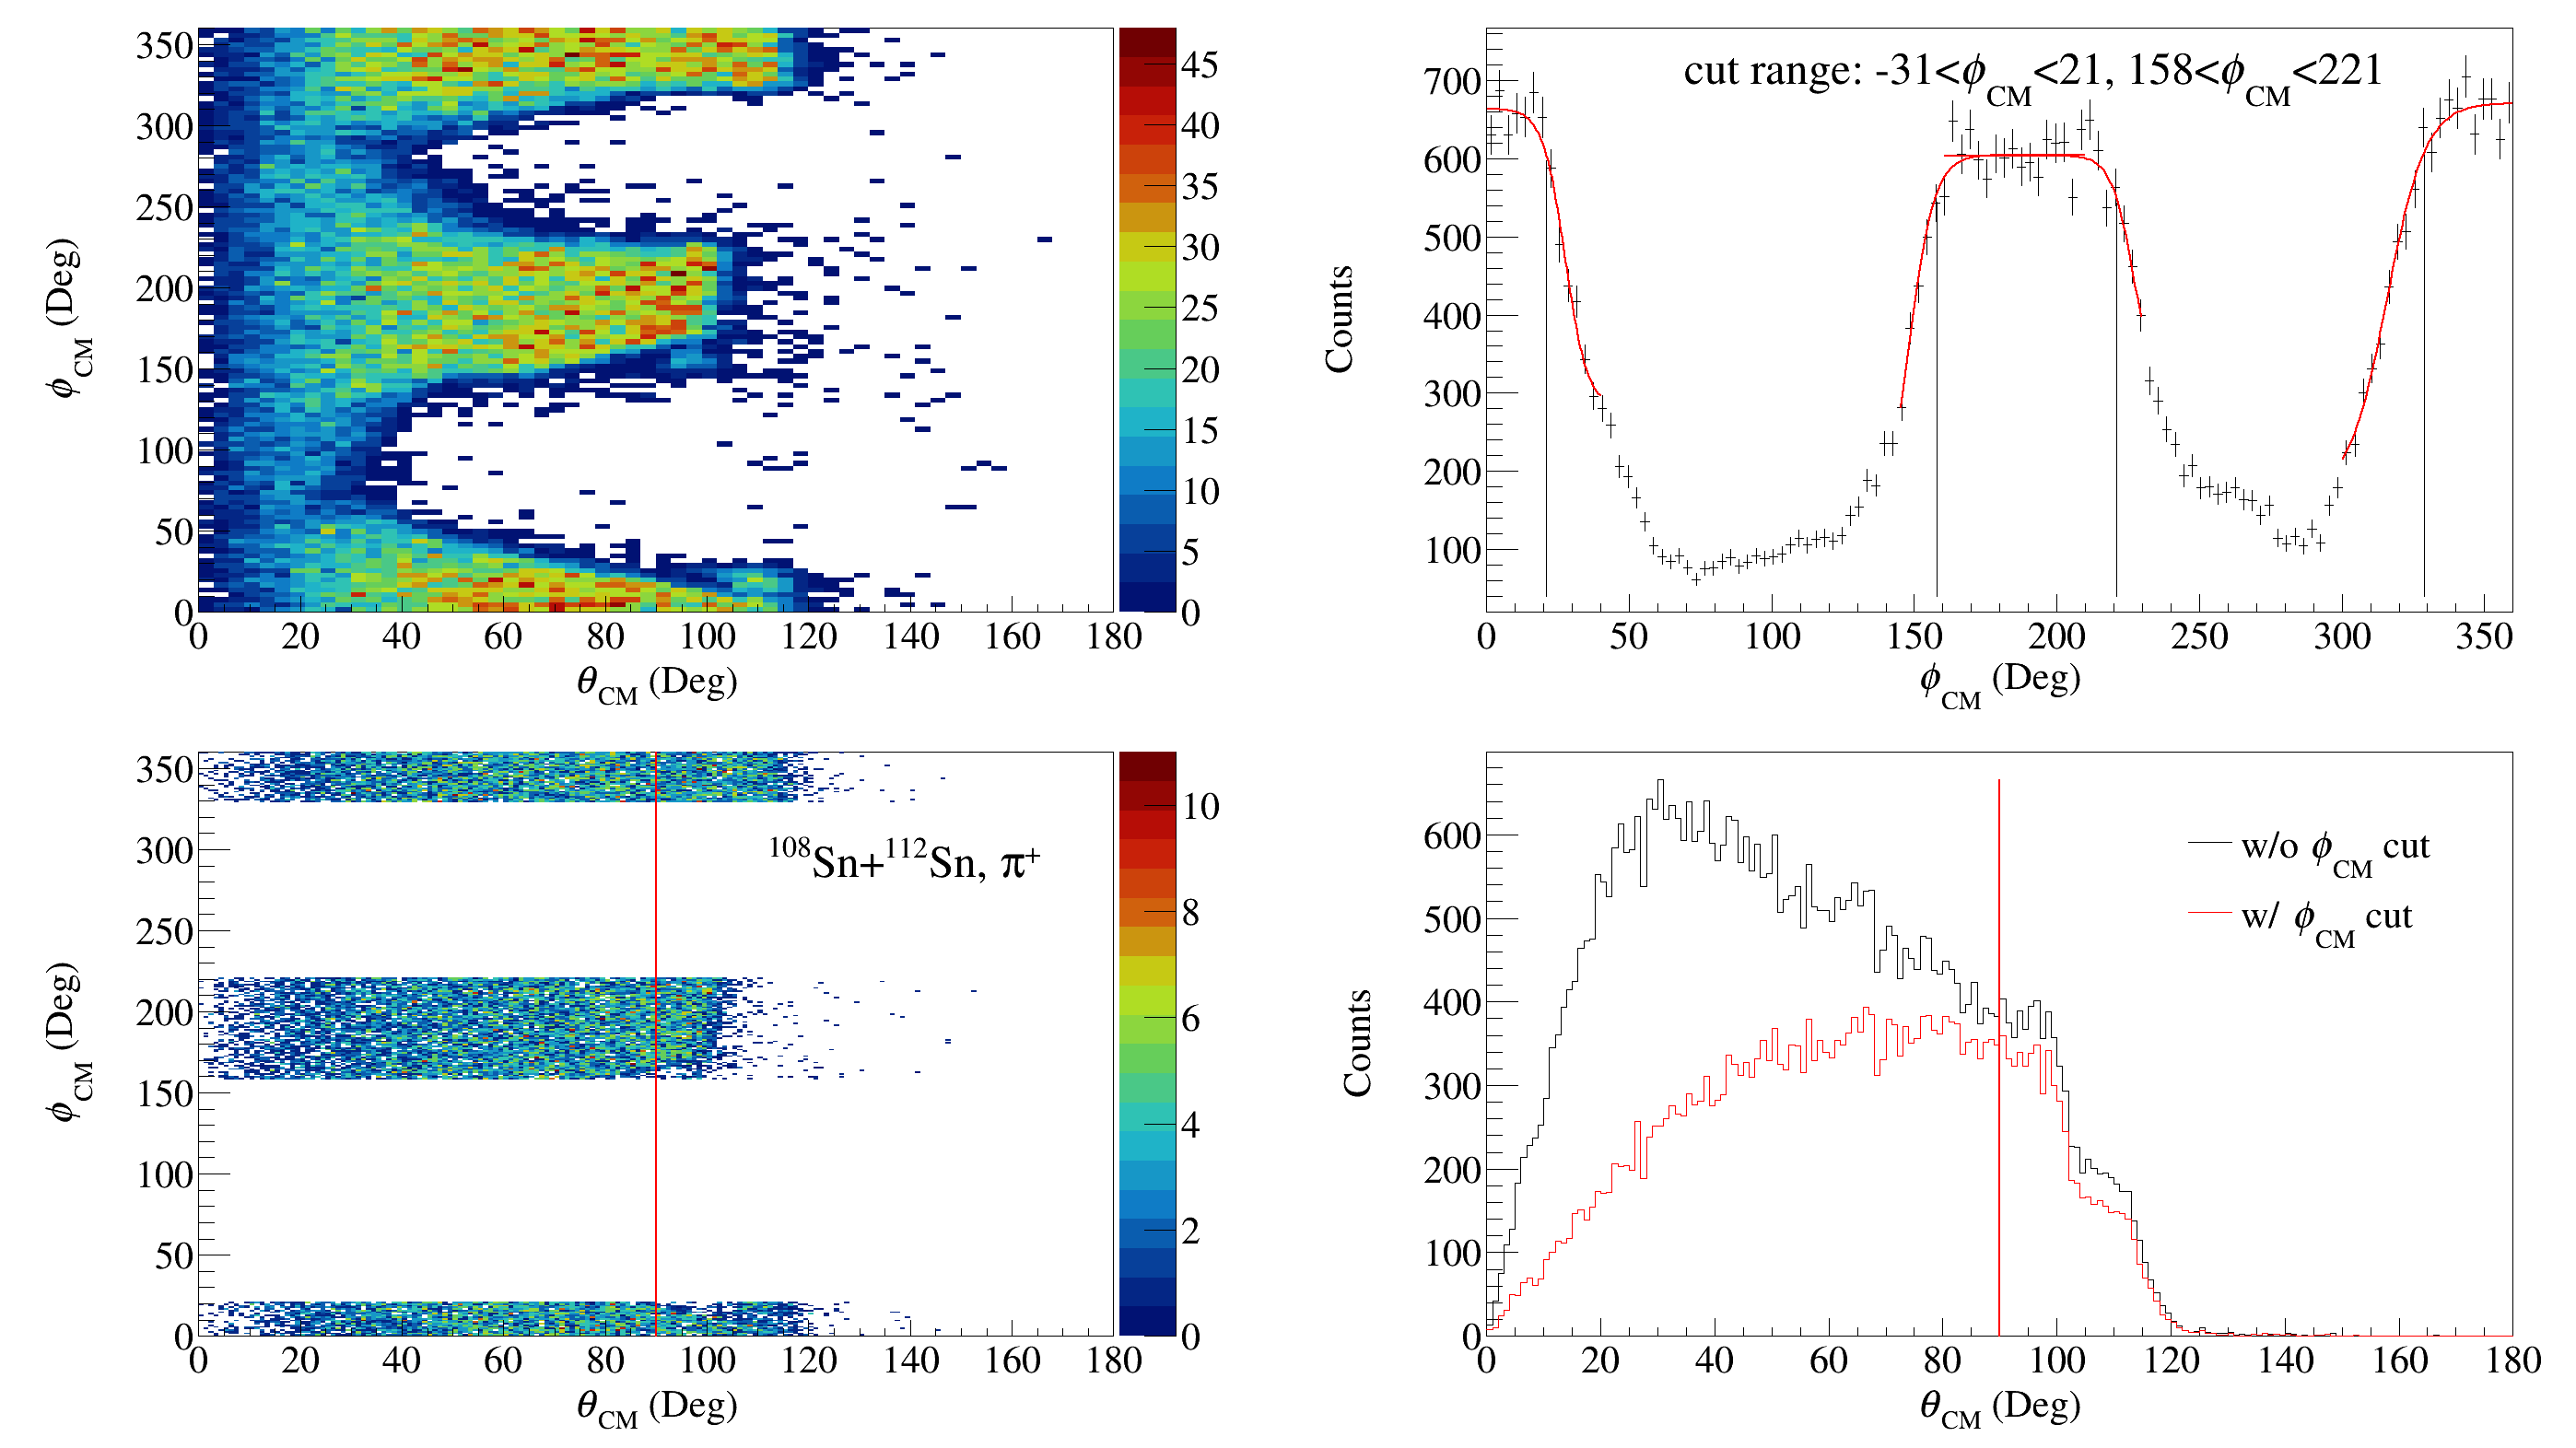
\includegraphics[width=\textwidth]{angularCut-pip-Sn108.png}
         \caption{$\pi^+$ angular cuts in the $\tin{108}{112}$ system. $\theta_{CM} < 90$ and < $\phi$ <}
         \label{fig:pip108angle}
     \end{subfigure}
     \hfill
     \begin{subfigure}[b]{0.49\textwidth}
         \centering
         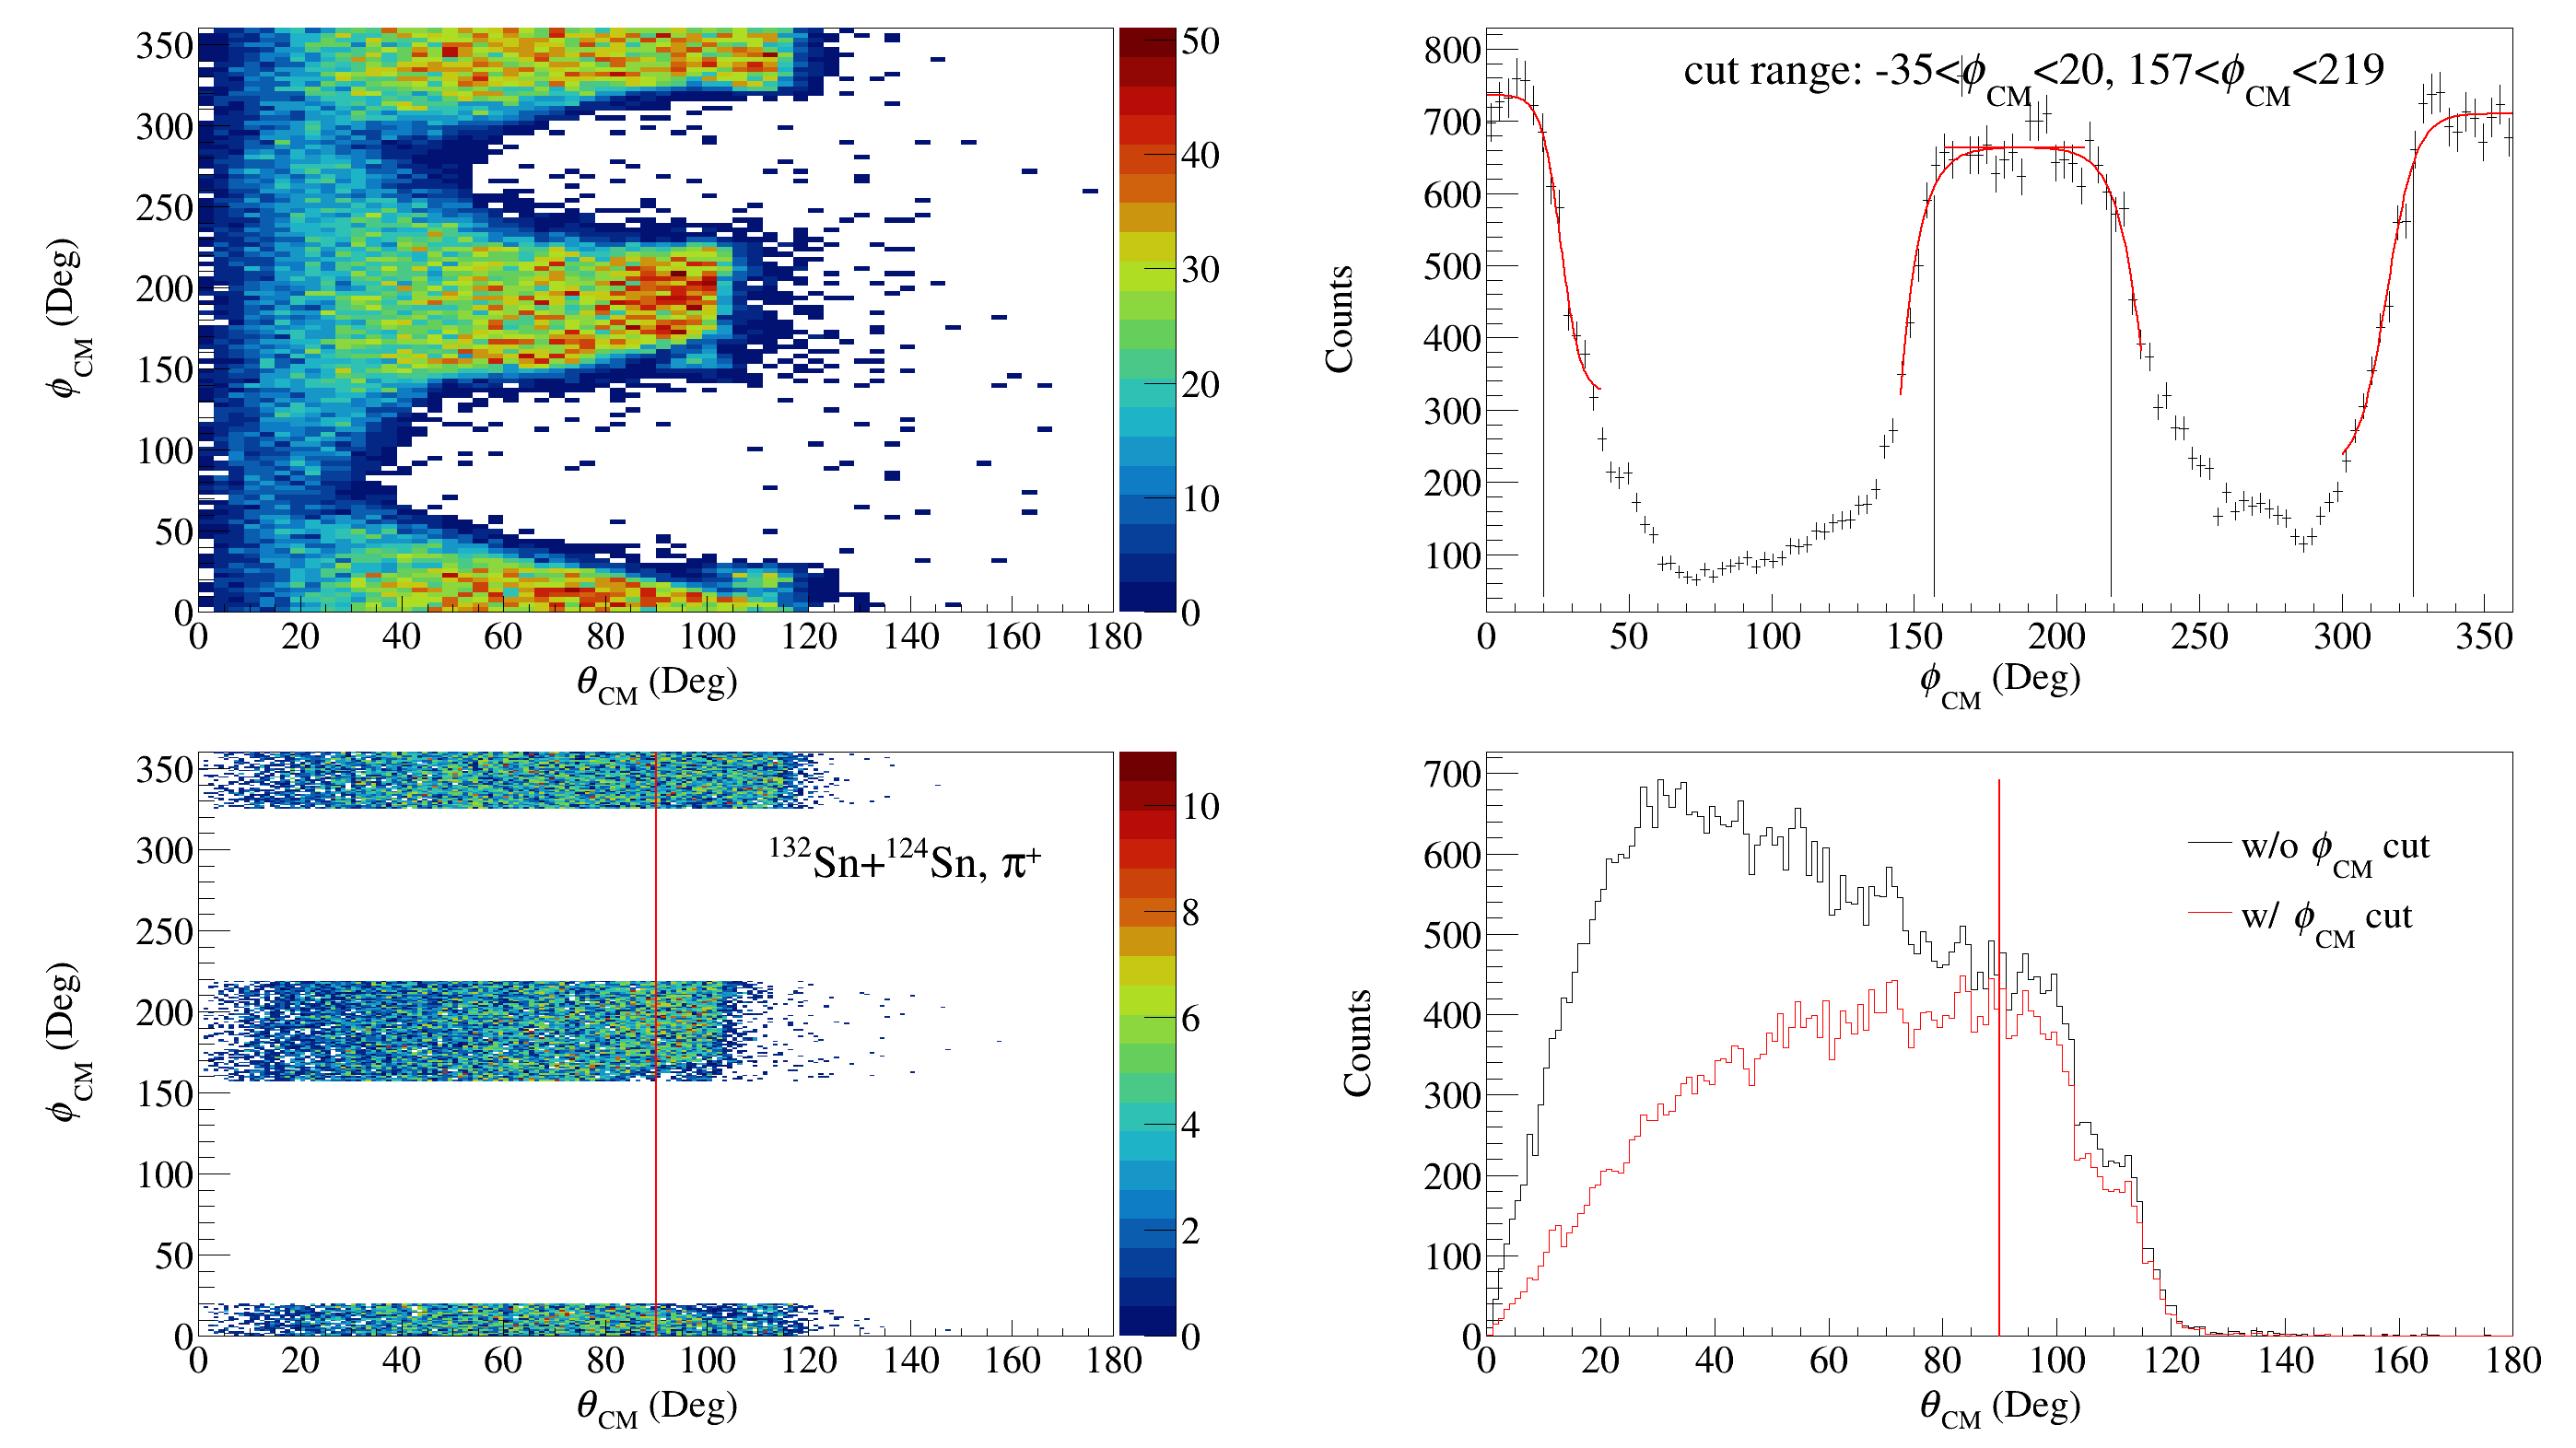
\includegraphics[width=\textwidth]{angularCut-pip-Sn132.png}
         \caption{$\pi^+$ angular cuts in the $\tin{132}{124}$ system. $\theta_{CM} < 90$ and < $\phi$ <}
         \label{fig:pip132angle}
     \end{subfigure}
        \caption{Measured $\pi^+$ angular distribution for the two spherical angles $\theta$ and $\phi$.}
        \label{fig:pip}
\end{figure}



 \begin{table*}[!htb]
 \centering
\ra{1.3}
\begin{tabular}{@{}ccc@{}}\toprule 
Particle Type & $\theta_{CM}$ cut & $\phi$ cut  \\ [0.5ex] 
 \midrule
$\pi^+$  & $\theta_{CM}$ < \ang{90}   &  \ang{-35} < $\phi$ < \ang{20} $\cap$ \ang{157} < $\phi$ < \ang{219}  \\
$\pi^-$  & $\theta_{CM}$ < \ang{90}   &  \ang{-40} < $\phi$ < \ang{25} $\cap$ \ang{158} < $\phi$ < \ang{212}   \\
 \bottomrule
\end{tabular}
\caption{Angular cuts for each system and particle type}
\label{tb:anglecuts}
\end{table*}



These regions can also be seen in the earlier discussion in the MC embedded efficiency in Figure~\ref{fig:pim_eff_ex}.  We could of course include a larger region where the efficiency is small, but not zero, but it is not good practice to  correct using small efficiency values. Instead we apply a reasonable $\phi$ cut in the good areas of reasonable efficiency and correct for the regions excluded from the cut. The solid angle covered by the cut is written as,

\begin{equation}
\Delta\Omega = \Delta\phi(\cos(\theta_1) - \cos(\theta_2)),
\end{equation}

where $\Delta\phi = (\phi_2 - \phi_1)$  and $\theta_{1,2}$ are the $\theta$ angle cuts, in units of \si{\radian}. The solid angle covered by the $\pi^-$ cuts is \SI{2.077}{\steradian} and for $\pi^+$ cuts \SI{2.042}{\steradian}. Assuming the pion emission is isotropic, we multiply each observed pion by a correction factor, $C_a$, to correct for the full 4$\pi$ angular coverage, 

\begin{equation}
C_a = \frac{4\pi}{\Delta\Omega},
\label{eq:acceptCorrFactor}
\end{equation}

for $\pi^+$ that is \num{6.15} and $\pi^-$ \num{6.05}. We assume the pion emission is isotropic for a couple of reasons. The symmetry of very central collisions is invariant with respects to any rotations. Also the mass of the pion is smaller than the nucleons mass and therefore collective motion leading to anisotropies would be small for the pion, i.e. most of the motion would be thermal. We also measured two systems $\tin{112}{124}$ and its inverse $\tin{124}{112}$. The forward emission in the $\tin{124}{112}$ system is really the same as the backward emission of the $\tin{112}{124}$ system and vice versa. It was shown for pions emitted in central collisions the forward and backward emission was the same \cite{jon}, proving that at least for central collisions pions are emitted isotropically to a good approximation. 


\subsection{Correcting Pion Spectra (Efficiency and Acceptance)}
\label{sec:corrSpectra}
To correct for the efficiency, we apply a track-by-track correction, where the efficiency of the i-th track $\epsilon_i$ is retrieved from the efficiency database, from the parameters discussed in Section~\ref{sec:efficiency}. The correction factor $C_i$ is defined as,

\begin{equation}
C_i = \epsilon_i^{-1}.
\label{eq:effCorrFactor}
\end{equation}

Each track that is identified as a pion as described in Section~\ref{sec:pid}, is then weighted by the correction factor $C_i$, when filling the histogram of any observable. In this way, we can correct for the efficiency on a track-by-track basis, allowing for any transformation of the track of interest into any observable, notably transforming from the lab frame into the center-of-mass (CM) frame. Before performing the transformation to the CM system, recall there is a small, but non-negligible, beam angle in the Lab frame discussed in Section~\ref{sec:beamangle}. First we rotate each event so that the beam will align with the z-axis. Doing so makes the transformation into the CM system much simpler to describe. If the beam direction is defined by a unit vector $\hat{b}$, we can define the rotation that rotates the beam into the z-axis as a rotation about an arbitrary vector $\hat{v} = \hat{b}\times\hat{z}$ where the angle between the two is given by $\cos \theta = \hat{b}\cdot\hat{z}$. A rotation with the angle $\theta$ is then applied around the vector $\hat{v}$.

Once all the events have been rotated to align with the z-axis, transforming from the Lab to the CM frame is done by a Lorentz transformation. The 4-momentum vector in the lab frame is defined as $\textbf{P} = (E/c,p_x,p_y,p_z)$. Where the corresponding Lorentz transform into the CM frame along the beam (z-axis) is defined as the Lorentz transformation matrix $A$,

\begin{equation}
A = \begin{pmatrix}
1 & 0 & 0 & 0\\
0 & 1 & 0 & 0\\
0 & 0 & \gamma & -\beta \gamma\\
0 & 0 & -\beta \gamma & \gamma
\end{pmatrix},
\end{equation}

where $\beta$, describes the velocity of the CM system, and $\gamma=\sqrt{1-\beta^2}^{-1}$. The parameter $\beta$ can be determined from the total momentum of the system in the Laboratory frame $P = \sqrt{ T_{P}^2 + 2M_{T}T_{T}}$ and the total energy of the system $E = T_{P} + M_{P} + M_{T}$ -- where $T_{P}$ is the projectile kinetic energy in the Lab frame, $M_{T}$, and $M_{P}$ are the total mass of the target and projectile, where $\beta = -P/E$; the (-) sign denotes the correct direction for transforming from the Lab to the CM frame. The transformation of each  track is defined as $p^{CM} = \textbf{A}p^{Lab}$.

\subsection{Pion Statistical Error}

The treatment of statistical error that will be discussed here applies to the total pion yield and the binned contents of the pion spectral ratio. The total pion multiplicity is defined as the number of pions per event. Accounting for all the corrections and cuts discussed above this can be expressed as, 

\begin{equation}
Y(\pi^\pm) = A\sum_{i} \frac{P(\pi)}{\epsilon_i},
\end{equation}

where $P(\pi)$ is the probability that a track is a pion described in Eq.~\ref{eq:pionProbs}, $\epsilon_i(p_{Lab}, \theta_{Lab})$ is the efficiency of particle $i$ given by its momentum $p_{Lab}$ and polar angle $\theta_{Lab}$ as discussed in Section~\ref{sec:efficiency}. The factor $A$ is a scale factor defined as,

\begin{equation}
 A = \frac{C_a}{N_{total}},
\end{equation}

where $N_{total}$ is the total number of events, $C_a$ is the correction factor accounting for the solid angle measured as given in Eq.~\ref{eq:acceptCorrFactor}. The statistical uncertainty is broken into two different parts, due to the way ROOT calculates the error of each histogram bin entry with the Sumw2() function, which calculates the error of each bin as,

\begin{equation}
{\delta b}^2 = \sum_i^{N_{\pi}} {\delta w_i}^2,
\end{equation}

where the weight of the bin is $w_i = A P(\pi) \epsilon_i^{-1}$. This still does not account for the efficiency error which was calculated using the MC embedding method. The efficiency class returns the error of each efficiency bin which scales like the total number of input track $\sqrt{N_{MC}}$. The extra error coming from the efficiency error can be expressed as,

\begin{equation}
{\delta \epsilon }^2 = A^2 \sum_i^{N_{\pi}} \left[ \left( \frac{P(\pi)^{\pi} }{\epsilon_i} \right)^2  \left(  \frac{P(\pi)^{\pi} }{\epsilon_i} \frac{\delta \epsilon_i}{\epsilon_i} \right)^2   \right]
\end{equation}

These two errors make up the total statistical error accounting for the measured number of particles, via Poisson statistics, and the efficiency error following error propagation. They are combined in quadrature such that the total error is $\delta \sigma^2 = \delta\epsilon^2 + \delta b^2$. The systematic error analysis is discussed in Appendix~\ref{sec:cutvar}. This discussion focuses on the systematics originating from the particular cuts we take in our analysis. As will be seen in the results section, the pion ratios seem to cancel out any of these effects and therefore any systematics introduced through our cuts need not be added into the total error bars. For the single particle yields some systematic error bars are added as guided by the cut variation analysis. 